\documentclass{beamer}

\usetheme{Boadilla}

\usepackage[english]{babel}
\usepackage[latin1]{inputenc}
\usepackage{latexsym}
\usepackage{slashed}
\usepackage{color}
\usepackage{tabularx}
\usepackage{booktabs}
\usepackage{threeparttable}
\usepackage{multirow}
\usepackage{colortbl}
\usepackage{rotating}
\usepackage{tikz}
\usepackage{appendixnumberbeamer}
\usepackage{feynmp}
\usepackage{graphicx}
\usepackage{epsfig}
\usepackage{mathtools}
\usepackage{wasysym}
\usepackage{mathrsfs}
\usepackage{scalerel}
\usepackage{feynmp}
\usepackage{tikz}
\usepackage{slashbox}
\usepackage{siunitx} % For correctly displayed SI units.
\sisetup{range-phrase = \text{--}} % For correctly displayed number ranges

\usetikzlibrary{shapes,arrows}

\tikzstyle{block}=[rectangle, draw, fill=blue!20, text width=9.5em, 
                   text centered, rounded corners, minimum height=2em, 
                   minimum width=10em]
\tikzstyle{line} =[draw, -latex']
\tikzstyle{decision} = [diamond, draw, fill=red!20, text width=7.5em, text centered,  inner sep=0pt, minimum height=2em, aspect=4]
%\tikzstyle{block} =  [rectangle, draw, fill=blue!20, text width=9.5em, text centered, rounded corners, minimum height=2em, minimum width=10em]
\tikzstyle{block1} =  [rectangle, draw, fill=blue!20, text width=14.5em, text centered, rounded corners, minimum height=2em, minimum width=15em]
\tikzstyle{cloud} = [draw, ellipse,fill=red!20, minimum height=2em]
\tikzstyle{inout} = [rectangle, draw, fill=green!20, text width=9.5em, text centered, rounded corners, minimum height=2em, minimum width=10em]
\tikzstyle{alert} = [rectangle, draw, fill=red!20, text width=9.5em, text centered, rounded corners, minimum height=2em, minimum width=10em]
\tikzstyle{large} =  [rectangle, draw, fill=blue!20, text width=34.5em, text centered, rounded corners, minimum height=2em, minimum width=35em]
\tikzstyle{decision1} = [diamond, draw, fill=red!20, text width=7.5em, text centered,  inner sep=0pt, minimum height=2em, aspect=2]

\usefonttheme[onlymath]{serif}

\def\bstar{{\color{blue}$\bigstar$}}
\def\bcirc{\raisebox{-1pt}{\scalebox{1.5}{\color{blue}$\circ$}}}
\def\rsquare{{\raisebox{-1pt}{\color{red}$\blacksquare$}}}

\definecolor{Red}{rgb}{1,0,0}
\definecolor{Green}{rgb}{0,1,0}
\definecolor{Blue}{rgb}{0,0,1}
\definecolor{Gray}{gray}{0.9}
\definecolor{springgreen}   {cmyk}{0.26, 0   , 0.76, 0   }
\definecolor{olivegreen}    {cmyk}{0.64, 0   , 0.95, 0.40}
\definecolor{emerald}       {cmyk}{1   , 0   , 0.50, 0   }
\definecolor{junglegreen}   {cmyk}{0.99, 0   , 0.52, 0   }
\definecolor{seagreen}      {cmyk}{0.69, 0   , 0.50, 0   }
\definecolor{green}         {cmyk}{1   , 0   , 1   , 0   }
\definecolor{forestgreen}   {cmyk}{0.91, 0   , 0.88, 0.12}
\definecolor{pinegreen}     {cmyk}{0.92, 0   , 0.59, 0.25}
\definecolor{sepia}         {cmyk}{0   , 0.83, 1   , 0.70}
\definecolor{cerulean}      {cmyk}{0.94, 0.11, 0   , 0   }
\definecolor{salmon}        {cmyk}{0   , 0.53, 0.38, 0   }
\definecolor{greenyellow}   {cmyk}{0.15, 0   , 0.69, 0   }
\definecolor{arsenic}       {rgb}{0.23, 0.27, 0.29}
\definecolor{britishracinggreen}{rgb}{0.0, 0.26, 0.15}
\definecolor{oxfordblue}{rgb}{0.0, 0.13, 0.28}
\definecolor{bostonuniversityred}{rgb}{0.8, 0.0, 0.0}
\definecolor{goldenyellow}{rgb}{1.0, 0.87, 0.0}


\newcommand{\la}{\left\langle}
\newcommand{\ra}{\right\rangle}
\newcommand{\lc}{\left[}
\newcommand{\rc}{\right]}
\newcommand{\lp}{\left(}
\newcommand{\rp}{\right)}
\newcommand{\be}{\begin{equation}}
\newcommand{\ee}{\end{equation}}
\newcommand{\dat}{\rm dat}
\newcommand{\net}{\rm net}
\newcommand{\tot}{\rm tot}
\newcommand{\val}{\rm val}
\newcommand{\gen}{\rm gen}
\newcommand{\tr}{\rm tr}
\def\l{\left}
\def\r{\right}

\newsavebox\feynbox
\newlength\tmplength
\newcommand\postfeynlabel[4]{%
  \setlength{\tmplength}{#2\ht#3}%
  \raisebox{#1\tmplength}{%
  \scaleto[1.7ex]{\raisebox{2.33pt}{\}}}{\tmplength}%
  \raisebox{\dimexpr.5\tmplength-.35\ht\strutbox}{#4}}%
}
\DeclareGraphicsRule{.1}{mps}{*}{} 
\DeclareGraphicsRule{.2}{mps}{*}{} 
\DeclareGraphicsRule{.3}{mps}{*}{}
\DeclareGraphicsRule{.4}{mps}{*}{}

\setbeamercovered{transparent}
\setbeamercolor{structure}{fg=oxfordblue}
\setlength{\tabcolsep}{3pt}
%\setbeamercolor{structure}{fg=black}

\title[Towards NNPDF4.0]{Towards NNPDF4.0:\\
The Structure of the Proton to One-Percent Accuracy
{\scriptsize PDF4LHC meeting}}
\date[March 22, 2021]{March 22, 2021}
\author[Emanuele R. Nocera]{Emanuele R. Nocera\\ {\scriptsize School of Physics and Astronomy, The University of Edinburgh\\ on behalf of the NNPDF Collaboration}}

\setbeamertemplate{frametitle}[default][center]

\begin{document}
\beamertemplatenavigationsymbolsempty

%TITLEPAGE-------------------------------------------------------------------------------------------------------
\begin{frame}
\titlepage
\vspace{0.7cm}
\begin{flushright}
 
\includegraphics[scale=0.15]{plots/nnpdf_logo_official}\\
\end{flushright}
\vspace{-0.7cm}
\end{frame}

%Slide01
\begin{frame}
 \frametitle{From NNPDF3.1 to NNPDF4.0}
 \footnotesize
 \begin{block}{}
  \centering
  Collaborative progress towards extending {\textcolor{red}{data}}, {\textcolor{blue}{theory}} and {\textcolor{forestgreen}{methodology}}\\
 \end{block}
 \scriptsize
 \renewcommand*{\arraystretch}{1.35}
 \begin{tabularx}{\textwidth}{lXr}
  06/2017 & {\bf NNPDF3.1}                                                              
          & {\tiny{[{\textcolor{salmon}{EPJ\,C77\,(2017)\,663}}]}}\\
  10/2017 & \textcolor{blue}{NNPDF3.1sx}: {\scriptsize PDFs with small-$x$ resummation}                                                
          & {\tiny{[{\textcolor{salmon}{EPJ\,C78\,(2018)\,321}}]}}\\
  12/2017 & \textcolor{blue}{NNPDF3.1luxQED}: {\scriptsize consistent photon PDF \`a la luxQED}                                            
          & {\tiny{[{\textcolor{salmon}{SciPost\,Phys.\,5\,(2018)\,008}}]}}\\
  02/2018 & \textcolor{red}{NNPDF3.1+ATLASphoton}: {\scriptsize inclusion of direct photon data}                                       
          & {\tiny{[{\textcolor{salmon}{EPJ\,C78\,(2018)\,470}}]}}\\
  12/2018 & \textcolor{forestgreen}{NNPDF3.1alphas}: {\scriptsize $\alpha_s$ from a correlated-replica method}                                     
          & {\tiny{[{\textcolor{salmon}{EPJ\,C78\,(2018)\,408}}]}}\\
  12/2018 & \textcolor{forestgreen}{NNPDF3.1nuc}: {\scriptsize heavy ion nuclear uncertainties in a fit}                                        
          & {\tiny{[{\textcolor{salmon}{EPJ\,C79\,(2019)\,282}}]}}\\
  05/2019 & \textcolor{forestgreen}{NNPDF3.1th}: {\scriptsize missing higher-order uncertainties in a fit}                                         
          & {\tiny{[{\textcolor{salmon}{EPJ\,C79\,(2019)\,838; ibid.\,931}}]}}\\
  07/2019 & \textcolor{forestgreen}{Gradient descent and hyperoptimisation in PDF fits} 
          & {\tiny{[{\textcolor{salmon}{EPJ\,C79\,(2019)\,676}}]}}\\
  12/2019 & \textcolor{red}{NNPDF3.1singletop}: {\scriptsize inclusion of single top $t$-channel data}                                          
          & {\tiny{[{\textcolor{salmon}{JHEP\,05\,(2020)\,067}}]}}\\
  05/2020 & \textcolor{red}{NNPDF3.1dijets}: {\scriptsize comparative study of single- and di-jets}                                             
          & {\tiny{[{\textcolor{salmon}{EPJ\,C80\,(2020)\,797}}]}}\\
  06/2020 & \textcolor{blue}{Positivity of $\overline{\rm MS}$ PDFs}                    
          & {\tiny{[{\textcolor{salmon}{JHEP\,11\,(2020)\,129}}]}}\\
  08/2020 & \textcolor{forestgreen}{PineAPPL}: {\scriptsize fast evaluation of EW$\times$QCD corrections}                                           
          & {\tiny{[{\textcolor{salmon}{JHEP\,12\,(2020)\,108}}]}}\\
  08/2020 & \textcolor{red}{NNPDF3.1strangeness}: {\scriptsize assessment of strange-sensitive data}                                        
          & {\tiny{[{\textcolor{salmon}{EPJ\,C80\,(2020)\,1168}}]}}\\
  11/2020 & \textcolor{forestgreen}{NNPDF3.1deu}: {\scriptsize deuteron uncertainties in a fit}                                        
          & {\tiny{[{\textcolor{salmon}{EPJ\,C81\,(2021)\,37}}]}}\\
  03/2021 & \textcolor{forestgreen}{Future tests}                                       
          & {\tiny{[{\textcolor{salmon}{arXiv:2103.08606}}]}}\\
  2021    & {\bf NNPDF4.0}                                                              
          & {\tiny{[{\textcolor{salmon}{to appear}}]}}\\
 \end{tabularx}
\end{frame}

%Slide02
\begin{frame}
 \frametitle{From NNPDF3.1 to NNPDF4.0}
 \footnotesize
 \centering
 \scriptsize
 \vspace{-0.1cm}
 \begin{equation}
  \mathcal{L}_{ij}(M_X,y,\sqrt{s})=\frac{1}{s}\sum_{i,j}
  f_i\left(\frac{M_Xe^y}{\sqrt{s}},M_X\right) 
  f_j\left(\frac{M_Xe^{-y}}{\sqrt{s}},M_X \right)
  \nonumber
 \end{equation}
 \footnotesize
 \begin{overlayarea}{\textwidth}{5.2cm}
  \only<1>
  {
  \centering
  \underline{SINGLET}\\
  \begin{columns}[c]
   \begin{column}{0.5\textwidth}
    \centering
        NNPDF3.1 (NNLO)\\
        \vspace{0.1cm}
        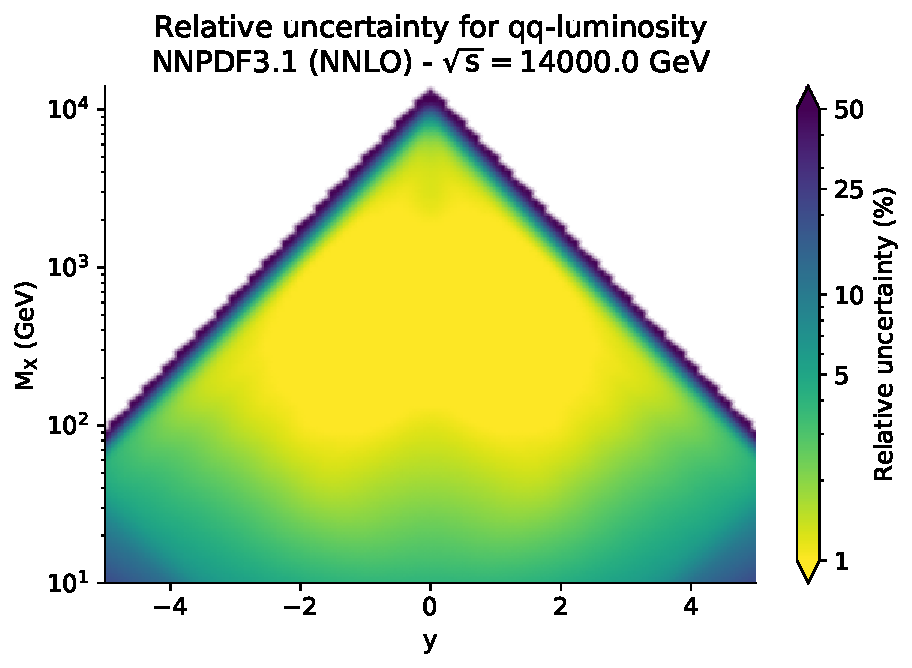
\includegraphics[width=\columnwidth]{plots/plot_lumi2d_uncertainty_NNPDF31_qq}\\
   \end{column}
   \begin{column}{0.5\textwidth}
    \centering
        NNPDF4.0 (NNLO)\\
        \vspace{0.1cm}
        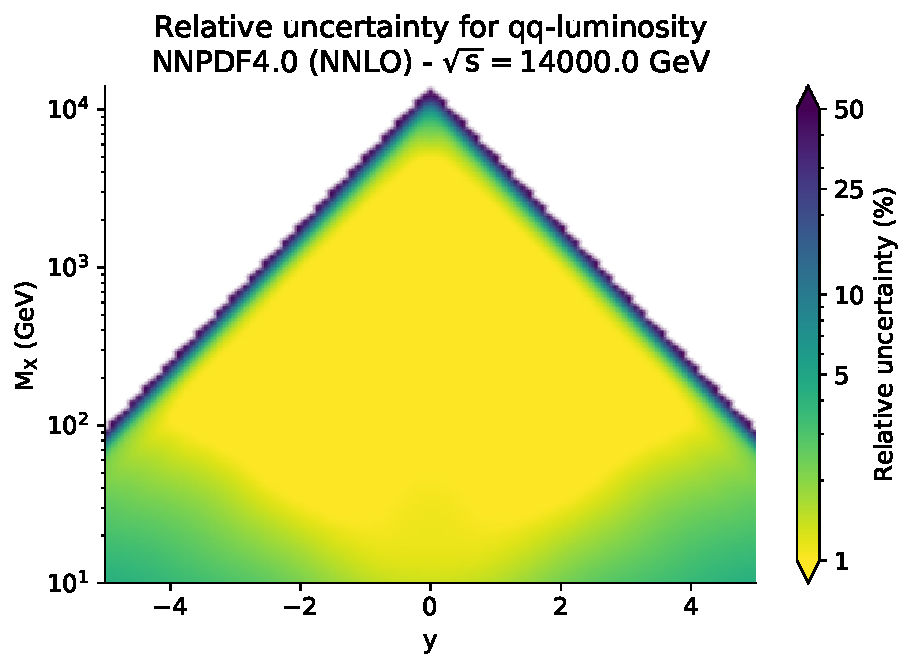
\includegraphics[width=\columnwidth]{plots/plot_lumi2d_uncertainty_NNPDF40_qq}\\    
   \end{column}
  \end{columns}
  }
  \only<2>
  {
  \centering
  \underline{SINGLET}\\
  \begin{columns}[c]
   \begin{column}{0.5\textwidth}
    \centering
        NNPDF3.1 (NNLO)\\
        \vspace{0.1cm}
        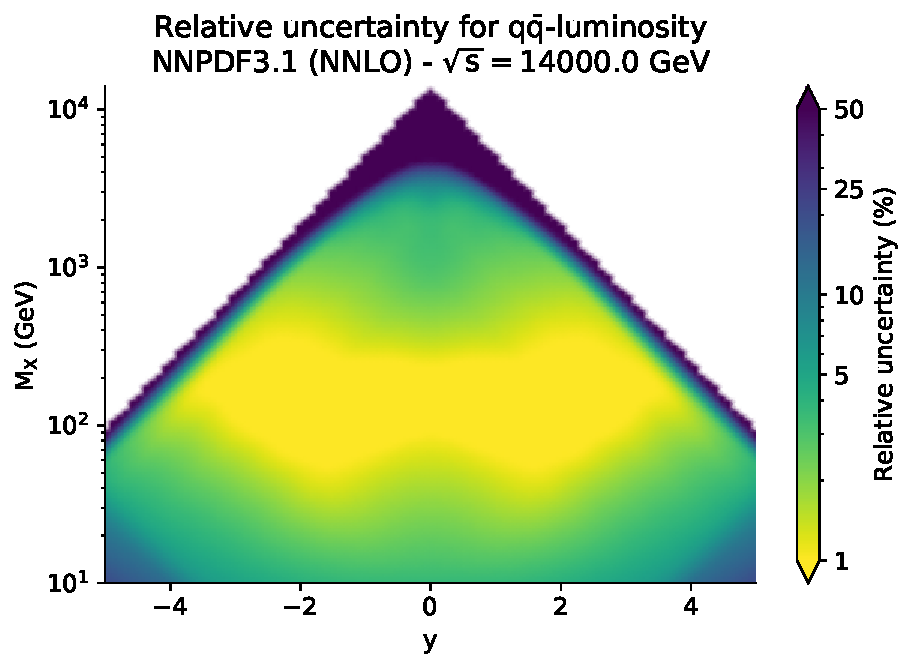
\includegraphics[width=\columnwidth]{plots/plot_lumi2d_uncertainty_NNPDF31_qqbar}\\
   \end{column}
   \begin{column}{0.5\textwidth}
    \centering
        NNPDF4.0 (NNLO)\\
        \vspace{0.1cm}
        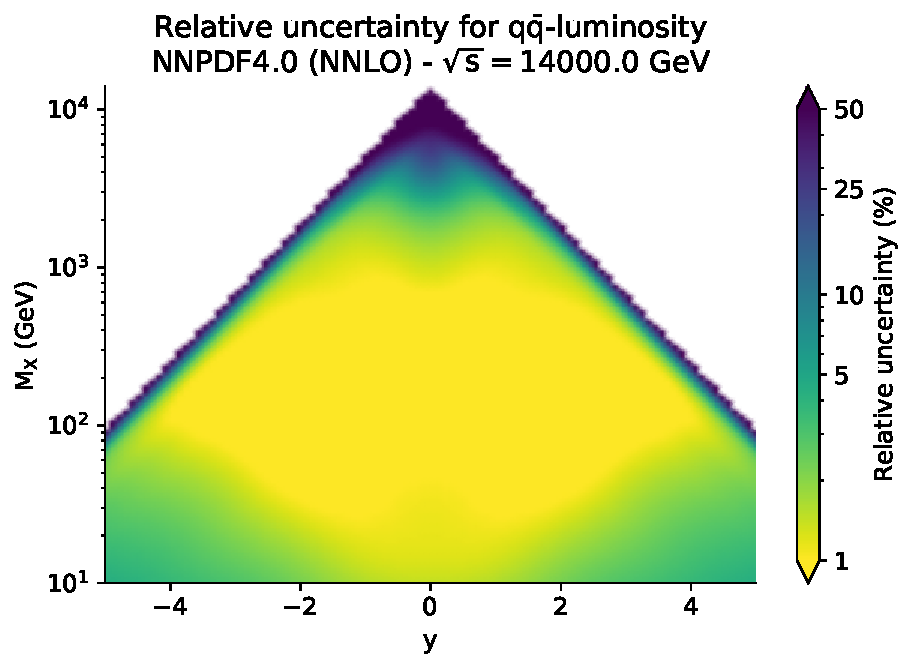
\includegraphics[width=\columnwidth]{plots/plot_lumi2d_uncertainty_NNPDF40_qqbar}\\    
   \end{column}
  \end{columns}  
  }
  \only<3>
  {
  \centering
  \underline{FLAVOURS}\\
  \begin{columns}[c]
   \begin{column}{0.5\textwidth}
    \centering
        NNPDF3.1 (NNLO)\\
        \vspace{0.1cm}
        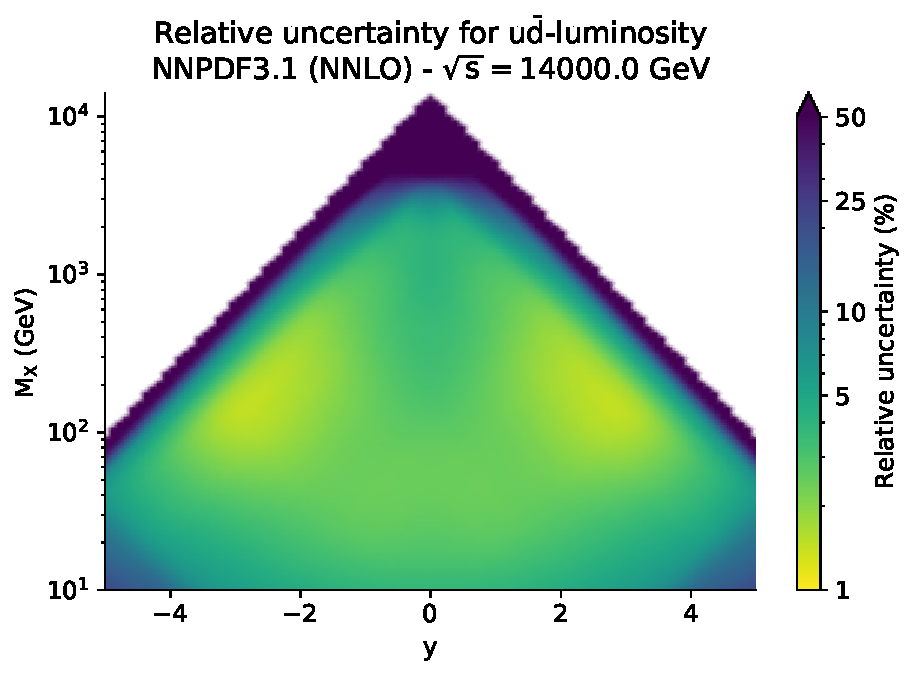
\includegraphics[width=\columnwidth]{plots/plot_lumi2d_uncertainty_NNPDF31_udbar}\\
   \end{column}
   \begin{column}{0.5\textwidth}
    \centering
        NNPDF4.0 (NNLO)\\
        \vspace{0.1cm}
        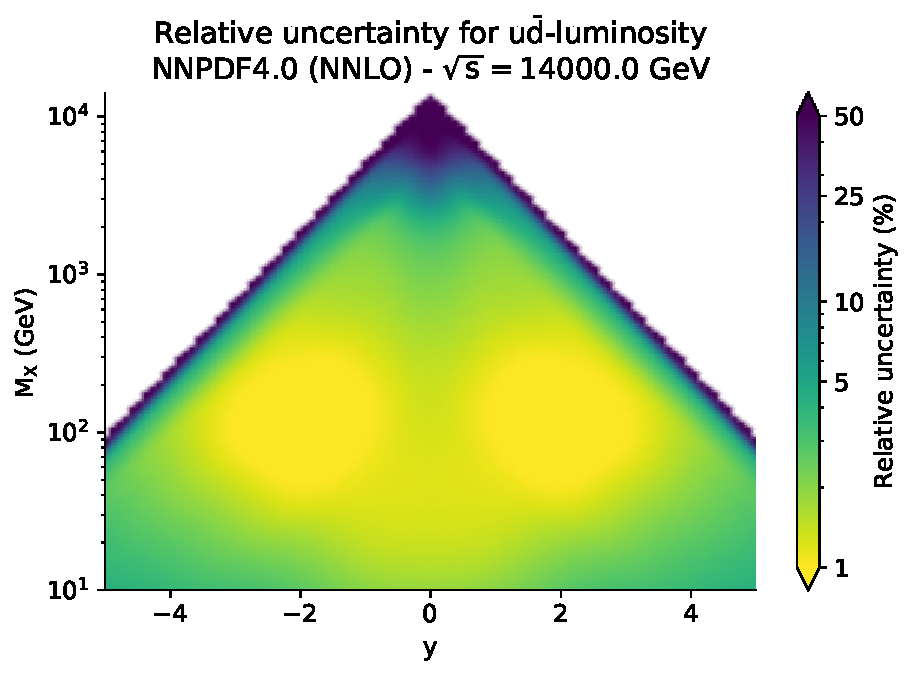
\includegraphics[width=\columnwidth]{plots/plot_lumi2d_uncertainty_NNPDF40_udbar}\\    
   \end{column}
  \end{columns}  
  } 
  \only<4>
  {
  \centering
  \underline{FLAVOURS}\\
  \begin{columns}[c]
   \begin{column}{0.5\textwidth}
    \centering
        NNPDF3.1 (NNLO)\\
        \vspace{0.1cm}
        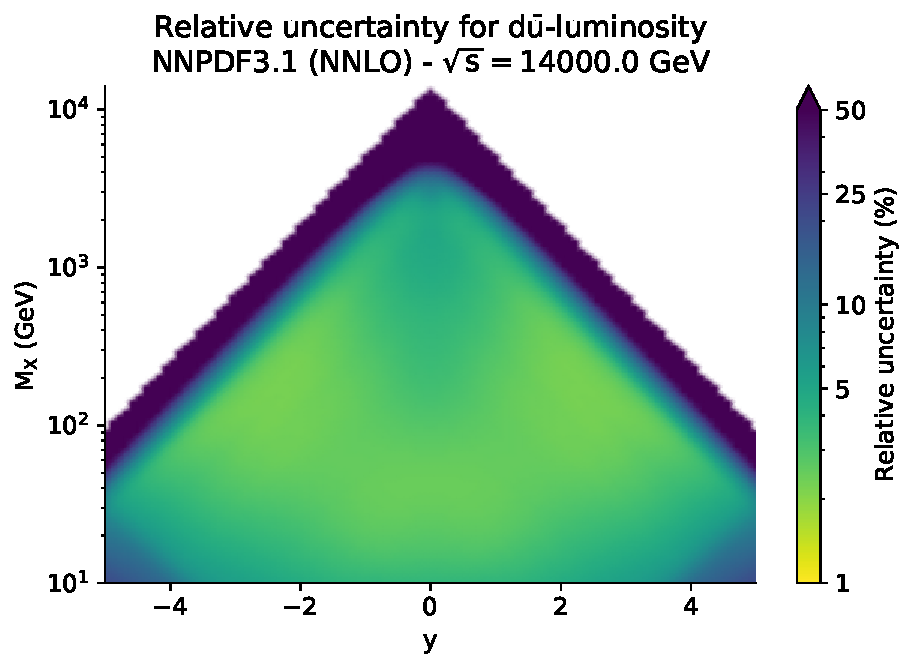
\includegraphics[width=\columnwidth]{plots/plot_lumi2d_uncertainty_NNPDF31_dubar}\\
   \end{column}
   \begin{column}{0.5\textwidth}
    \centering
        NNPDF4.0 (NNLO)\\
        \vspace{0.1cm}
        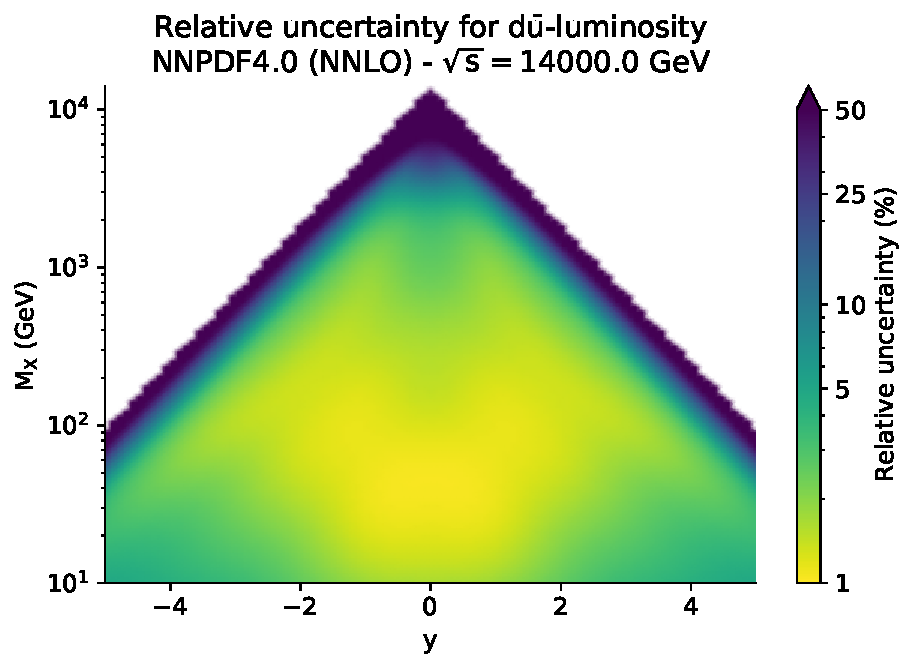
\includegraphics[width=\columnwidth]{plots/plot_lumi2d_uncertainty_NNPDF40_dubar}\\    
   \end{column}
  \end{columns}  
  }   
  \only<5>
  {
  \centering
  \underline{GLUON}\\
  \begin{columns}[c]
   \begin{column}{0.5\textwidth}
    \centering
        NNPDF3.1 (NNLO)\\
        \vspace{0.1cm}
        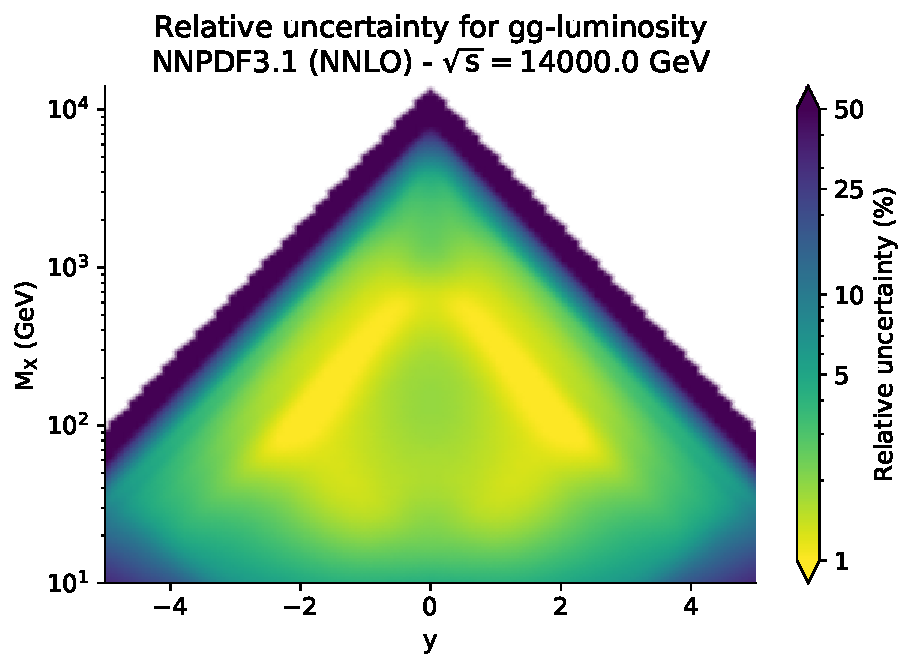
\includegraphics[width=\columnwidth]{plots/plot_lumi2d_uncertainty_NNPDF31_gg}\\
   \end{column}
   \begin{column}{0.5\textwidth}
    \centering
        NNPDF4.0 (NNLO)\\
        \vspace{0.1cm}
        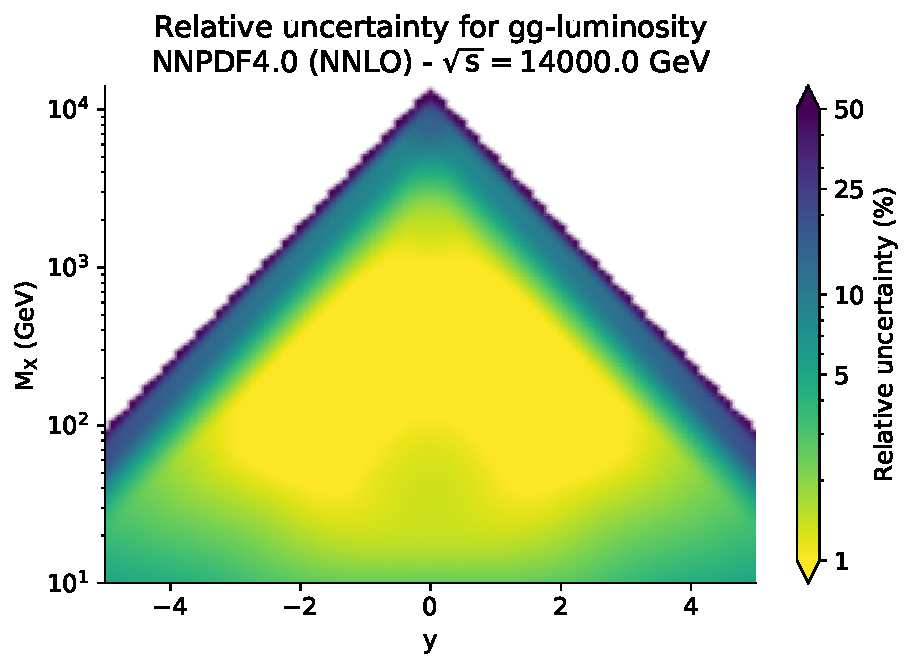
\includegraphics[width=\columnwidth]{plots/plot_lumi2d_uncertainty_NNPDF40_gg}\\    
   \end{column}
  \end{columns}  
  } 
  \only<6>
  {
  \centering
  \underline{GLUON}\\
  \begin{columns}[c]
   \begin{column}{0.5\textwidth}
    \centering
        NNPDF3.1 (NNLO)\\
        \vspace{0.1cm}
        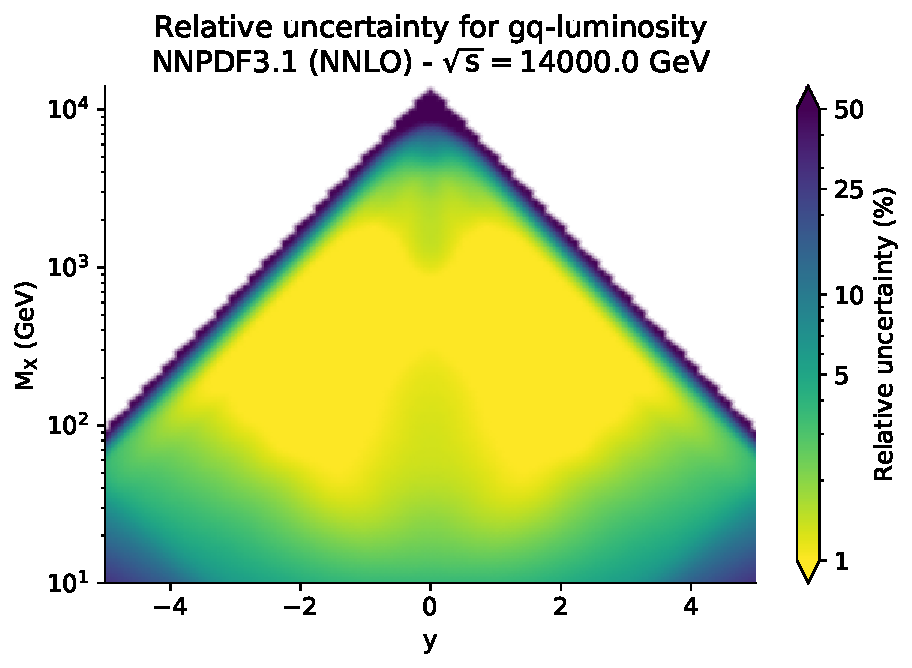
\includegraphics[width=\columnwidth]{plots/plot_lumi2d_uncertainty_NNPDF31_gq}\\
   \end{column}
   \begin{column}{0.5\textwidth}
    \centering
        NNPDF4.0 (NNLO)\\
        \vspace{0.1cm}
        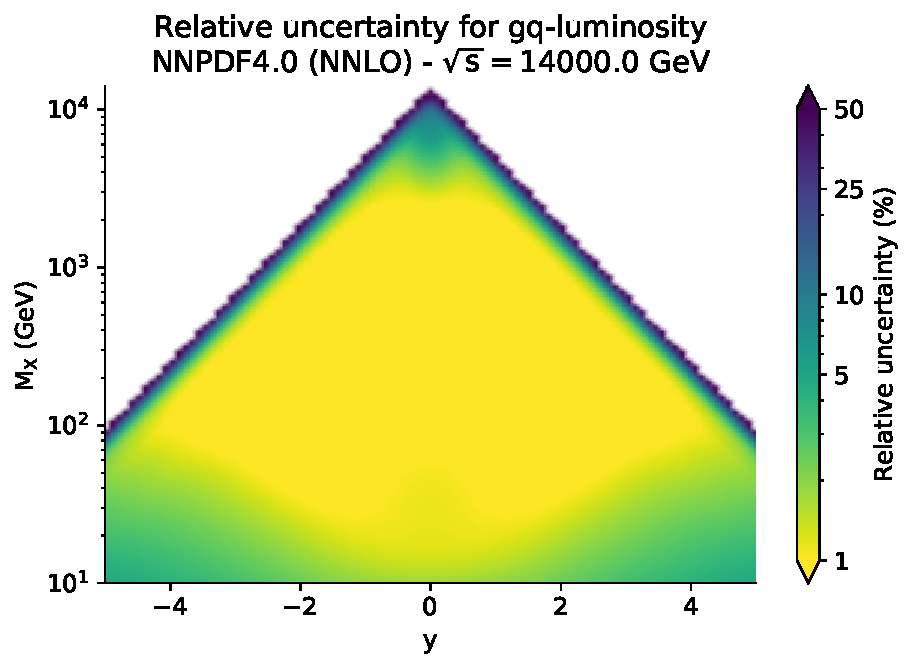
\includegraphics[width=\columnwidth]{plots/plot_lumi2d_uncertainty_NNPDF40_gq}\\    
   \end{column}
  \end{columns}  
  }   
 \end{overlayarea}
 \begin{alertblock}{}
  \centering
  Steady progress towards 1\% relative uncertainties on $\mathcal{L}_{ij}$ on a broad kinematic range\\
 \end{alertblock}
 \vspace{-0.1cm}
 \begin{block}{}
  \centering
  How are we getting there?\\
 \end{block}
\end{frame}

%Slide03
\begin{frame}
 \frametitle{NNPDF4.0: data set extension}
 \footnotesize
 \centering
 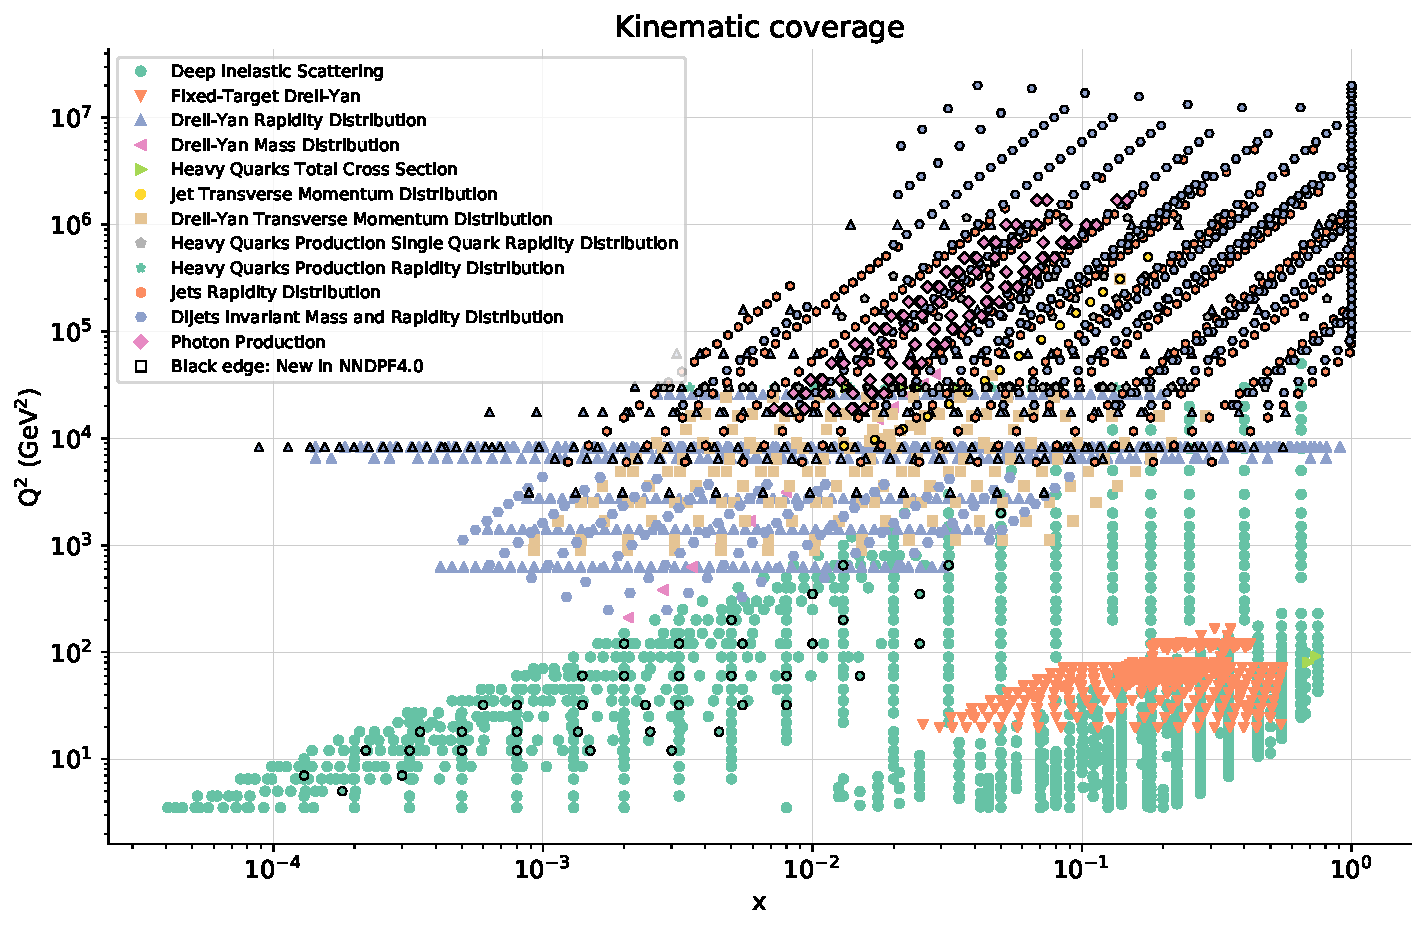
\includegraphics[width=\textwidth]{plots/Markers0_plot_xq2}\\
 $\mathcal{O}(50)$ data sets investigated; $\mathcal{O}(400)$ data points more in NNPDF4.0 than in NNPDF3.1
\end{frame}

%Slide04
\begin{frame}
 \frametitle{New data sets in NNPDF4.0}
 \tiny
 \vspace{0.1cm}
 %\renewcommand*{\arraystretch}{1.15}
 \begin{tabularx}{\textwidth}{llXr}
 \toprule
 Process    & Experiment & Description                                         & Reference\\
 \midrule
 DIS        
            & HERA        & Combined reduced $c$ and $b$ cross sections                      & [{\textcolor{salmon}{EPJ\,C78\,(2018)\,473}}]\\
            & NOMAD$^*$   & $\mathcal{R}_{\mu\mu}(E)=\sigma_{\mu\mu}(E)/\sigma_{\rm CC}(E)$  & [{\textcolor{salmon}{NPB\,876\,(2013)\,339}}]\\
 DY         
            & ATLAS       & $W,Z$ central/forward rapidity distr., {\bf 7~TeV}    & [{\textcolor{salmon}{EPJ\,C77\,(2017)\,367}}]\\
            & ATLAS       & $\{m_{\ell\ell},|y_{\ell\ell}|\}$ high-mass distribution, {\bf 8~TeV} & [{\textcolor{salmon}{JHEP\,08\,(2016)\,009}}]\\
            & ATLAS       & $W$ and $Z$ total cross section, {\bf 13~TeV}                    & [{\textcolor{salmon}{PLB\,759\,(2016)\,601}}]\\
            & LHCb        & $y_Z$ distribution, $2e$ and $2\mu$, {\bf 13~TeV}                & [{\textcolor{salmon}{JHEP\,09\,(2016)\,136}}]\\  
 $W$+c 
            & ATLAS$^\dag$& $|\eta^\ell|$ distribution  {\bf 7~TeV}                          & [{\textcolor{salmon}{JHEP\,05\,(2014)\,068}}]\\
            & CMS$^\dag$  & $|\eta^\mu|$ distribution  {\bf 13~TeV}                          & [{\textcolor{salmon}{EPJ\,C79\,(2019)\,269}}]\\ 
 single-jet 
            & ATLAS       & $\{p_T, |y|\}$ distribution, {\bf 8~TeV}                         & [{\textcolor{salmon}{JHEP\,09\,(2017)\,020}}]\\
 $t\bar{t}$ 
            & CMS         & total inclusive cross section, {\bf 5~TeV}                       & [{\textcolor{salmon}{JHEP\,03\,(2018)\,115}}]\\
            & CMS         & normalised $\{m_{t\bar{t}},y_t\}$ distribution, {\bf 8~TeV}      & [{\textcolor{salmon}{EPJ\,C77\,(2017)\,459}}]\\
            & CMS         & normalised $y_t$ distribution (dilepton), {\bf 13~TeV}           & [{\textcolor{salmon}{JHEP\,02\,(2019)\,149}}]\\
            & CMS         & normalised $y_t$ distribution (lepton+jet), {\bf 13~TeV}         & [{\textcolor{salmon}{PRD\,97\,(2018)\,112003}}]\\ 
 \midrule
 \alert{single top} 
            & ATLAS       & $R_t$ {\bf 7, 8, 13~TeV}                                         & [{\textcolor{salmon}{JHEP\,04\,(2017)\,086}}]\\
            & ATLAS       & normalised $y_t$ and $y_{\bar{t}}$ distributions, {\bf 7, 8~TeV} & [{\textcolor{salmon}{PRD\,90\,(2014)\,112006; EPJ\,C77\, (2017)\,531}}]\\
            & CMS         & $t+\bar{t}$ cross section, {\bf 7~TeV}                           & [{\textcolor{salmon}{JHEP\,12\,(2012)\,035}}]\\
            & CMS         & $R_t$ {\bf 8, 13~TeV}                                            & [{\textcolor{salmon}{JHEP\,06\,(2014)\,090; PLB\,772\,(2017)\,752}}]\\
 \alert{$W$+jet}    
            & ATLAS       & $p_T$ distribution, {\bf 8~TeV}                                  & [{\textcolor{salmon}{JHEP\,05\,(2018)\,077}}]\\        
 \alert{isolated photon} 
            & ATLAS       & $\{E_T^\gamma,|\eta^\gamma|\}$ distribution, {\bf 13~TeV}        & [{\textcolor{salmon}{PLB\,770\,(2017)\,473}}]\\     
 \alert{di-jets}    
            & ATLAS       & $\{m_{12},y^*\}$ distribution {\bf 7~TeV}                        & [{\textcolor{salmon}{JHEP\,05\,(2014)\,059}}]\\
            & CMS         & $\{m_{12},|y_{\rm max}|\}$ distribution {\bf 7~TeV}              & [{\textcolor{salmon}{PRD\,87\,(2013)\,112002}}]\\
            & CMS         & $\{p_{\rm T,avg},y_b,y^*\}$ distribution {\bf 8~TeV}             & [{\textcolor{salmon}{EPJ\,C77\,(2017)\,746}}]\\           
 \alert{DIS+jets}   
            & H1$^*$      & Single- and di-jet differential distributions                         & [{\textcolor{salmon}{EPJ\,C75\,(2015)\,65; C77\,(2017)\,215}}]\\
 \bottomrule 
 \multicolumn{3}{l}{$^*$Under consideration via reweighting.} &
 \multicolumn{1}{l}{$^\dag$Only NLO fit.}\\
 \multicolumn{4}{l}{Processes highlighted in \alert{red} correspond to processes NOT in NNPDF3.1.}\\
 \end{tabularx}
 \vspace{-0.2cm}
 \scriptsize
 \begin{block}{}
  \centering
  Selection of data sets based on weighted fits (see Z. Kassabov)\\
  {\scriptsize Example: D0 $W$ electron asymmetry no longer in NNPDF4.0}\\
 \end{block}
\end{frame}

%Slide05
\begin{frame}
 \frametitle{NNPDF4.0: theoretical and methodological features}
 \footnotesize
 \centering
 \begin{block}{}
  \centering
  Mostly covered in the previous NNPDF talk; here I summarise the main points\\
 \end{block}
 \begin{itemize}
  \item \underline{Refined} theoretical framework\\
  {\scriptsize $\rightarrow$ nuclear uncertainties for both deuteron and heavy nuclei included by default}\\
  {\scriptsize $\rightarrow$ NNLO charm-quark massive corrections implemented (a bug in the NLO corrected)}\\
  {\scriptsize $\rightarrow$ EW corrections not included to ensure consistency with data, but carefully checked}\\  
  {\scriptsize $\rightarrow$ charm PDF parametrised on the same footing as other PDFs}\\
  \item \underline{Improved} implementation of PDF properties\\
  {\scriptsize $\rightarrow$ extended positivity constraints for light quark/antiquark and gluon PDFs}\\
  {\scriptsize $\rightarrow$ extended integrability constraints of non-singlet light quark PDF combinations}\\
  \item \underline{New} PDF parametrisation and optimisation \\
  {\scriptsize $\rightarrow$ single neural network to parametrise eight independent PDF combinations}\\
  {\scriptsize $\rightarrow$ new optimisation strategy based on gradient descent rather than genetic algorithms}\\
  {\scriptsize $\rightarrow$ scan of the hyperparameter space to find the optimal minimisation settings}\\
  \item \underline{Complete} statistical validation of PDF uncertainties\\
  {\scriptsize $\rightarrow$ (multi-)closure tests to validate PDF uncertainties in the data region}\\
  {\scriptsize $\rightarrow$ future tests to check the sensibleness of PDF uncertainties in extrapolation regions}\\
  \item \underline{More efficient} compression tool for PDF set delivery 
 \end{itemize}
\end{frame}

%Slide06
\begin{frame}
 \frametitle{NNPDF4.0: Fit quality}
 \footnotesize
 \centering
 \begin{columns}[c]
  \begin{column}{0.5\textwidth}
  \tiny
  \renewcommand*{\arraystretch}{1.1}
   \begin{tabularx}{\columnwidth}{Xrc}
   \toprule
   Data set                   & $N_{\rm dat}$ & $\chi^2/N_{\rm dat}$ \\
   \midrule
   Fixed-target DIS           & 1881 & 1.10 \\
   HERA                       & 1208 & 1.21 \\
   \ $\sigma_c$               &   37 & 2.11 \\
   \ $\sigma_b$               &   26 & 1.48 \\
   Fixed-target Drell-Yan     &  189 & 1.00 \\
   CDF                        &   28 & 1.31 \\
   D0                         &   37 & 1.00 \\
   ATLAS                      &  621 & 1.18 \\
   \ Drell-Yan, 7, 8, 13~TeV  &  153 & 1.32 \\
   \ $W$+jet, 8~TeV           &   32 & 1.15 \\
   \ single top, 7, 8, 13~TeV &   14 & 0.36 \\
   \ di-jets, 7~TeV           &   90 & 1.93 \\
   \ jets, 8~TeV              &  171 & 0.61 \\
   \ top pair, 7, 8, 13~TeV   &   16 & 2.30 \\
   \ $Zp_T$, 8~TeV            &   92 & 0.86 \\
   \ direct photon, 13~TeV    &   53 & 0.72 \\
   CMS                        &  411 & 1.40 \\
   \ Drell-Yan, 7, 8~TeV      &  154 & 1.34 \\
   \ single top, 7, 8, 13~TeV &    3 & 0.43 \\
   \ di-jets, 7~TeV           &   54 & 1.67 \\
   \ di-jets, 8~TeV           &  122 & 1.50 \\
   \ top pair, 5, 7, 8~TeV    &   29 & 0.84 \\
   \ top pair, 13~TeV         &   21 & 0.67 \\
   \ $Zp_T$, 8~TeV            &   28 & 1.42 \\
   LHCb                       &  116 & 1.53 \\
   \midrule
   Total                      & 4491 & 1.17 \\
   \bottomrule 
   \end{tabularx}
  \end{column}
  \begin{column}{0.5\textwidth}
   \centering
   \footnotesize
   Overall good description of the data sets\\
   \vspace{0.2cm}
   Two exceptions:\\
   HERA $\sigma_c$ and ATLAS top pair\\
   \vspace{0.2cm}
   Weighted fits analysis:\\
   {\scriptsize in case of HERA $\sigma_c$:}\\
   {\scriptsize lack of small-$x$ resummation}\\
   \vspace{0.2cm}
   {\scriptsize in case of ATLAS top pair:\\ slight tension with (di-jet) data sets}\\
   {\scriptsize poor fit if all distributions are included}\\
   {\scriptsize normalised rapidity distributions retained}\\
   {\scriptsize although their $\chi^2/N_{\rm dat}$ of order 3}\\
   {\scriptsize CMS top pair data almost insensitive to all this}\\
   \vspace{0.2cm}
   General remark:\\
   {\scriptsize as statistical uncertainties become smaller}\\
   {\scriptsize a good control of systematic uncertainties}\\ 
   {\scriptsize and their correlations becomes fundamental}\\ 
   {\scriptsize to interpret the sensibleness of the fit}\\
  \end{column}
 \end{columns}
\end{frame}

%Slide07
\begin{frame}
 \frametitle{From NNPDF3.1 to NNPDF4.0}
 \footnotesize
 \centering
 \begin{columns}[c]
  \begin{column}{0.5\textwidth}
   \begin{overlayarea}{\columnwidth}{4cm}
    \only<1>
    {
     \centering
     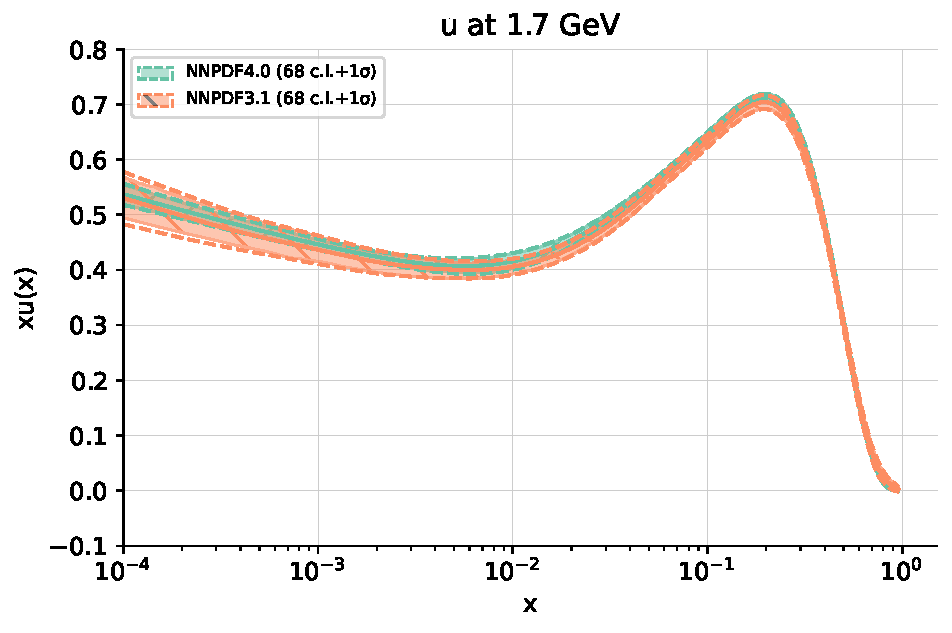
\includegraphics[width=\columnwidth]{plots/u_fit_1}\\    
    }
    \only<2>
    {
     \centering
     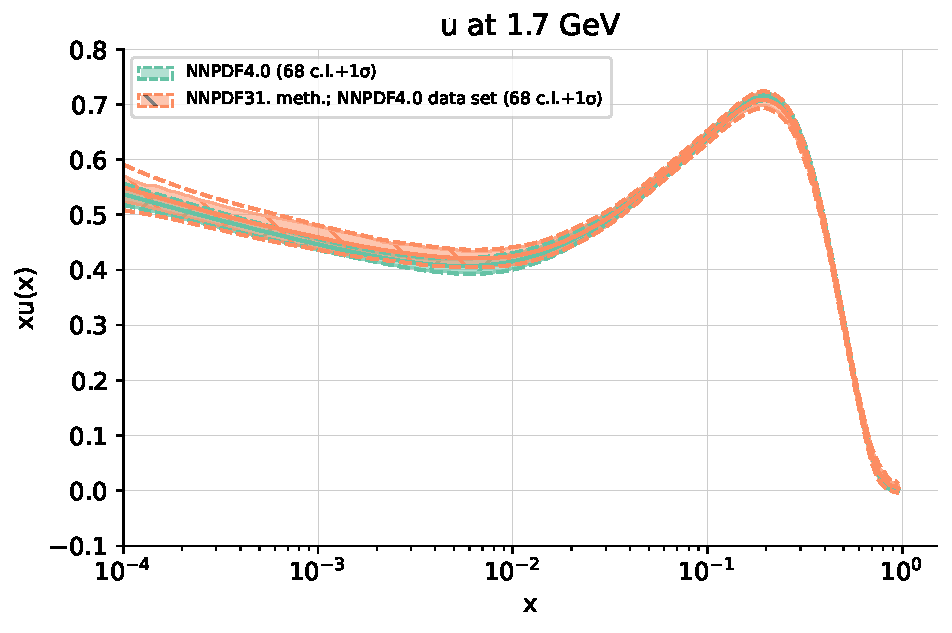
\includegraphics[width=\columnwidth]{plots/u_fit_2}\\    
    }
   \end{overlayarea}
  \end{column}
  \begin{column}{0.5\textwidth}
   \begin{overlayarea}{\columnwidth}{4cm}
    \only<1>
    {
     \centering
     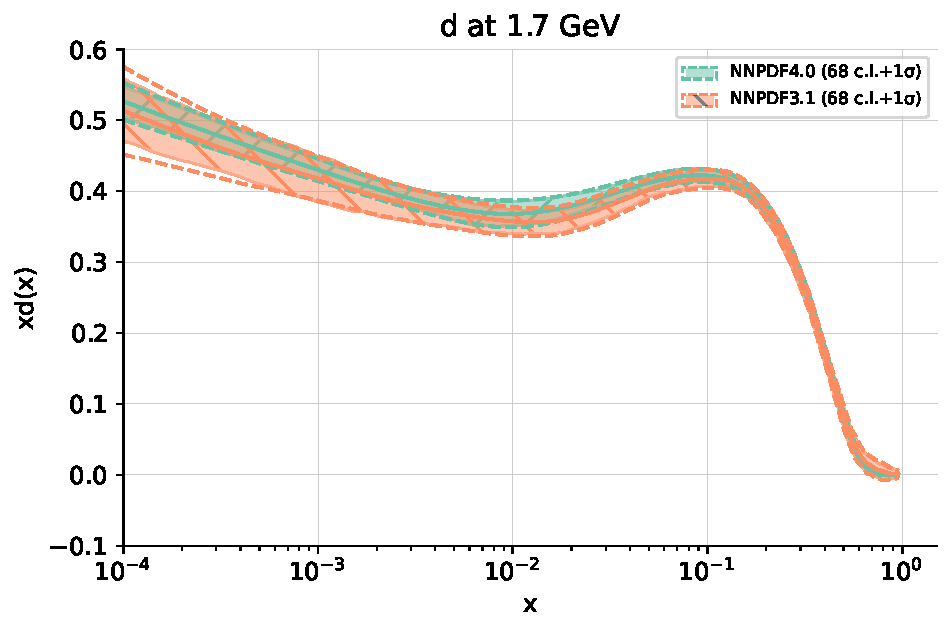
\includegraphics[width=\columnwidth]{plots/d_fit_1}\\    
    }
    \only<2>
    {
     \centering
     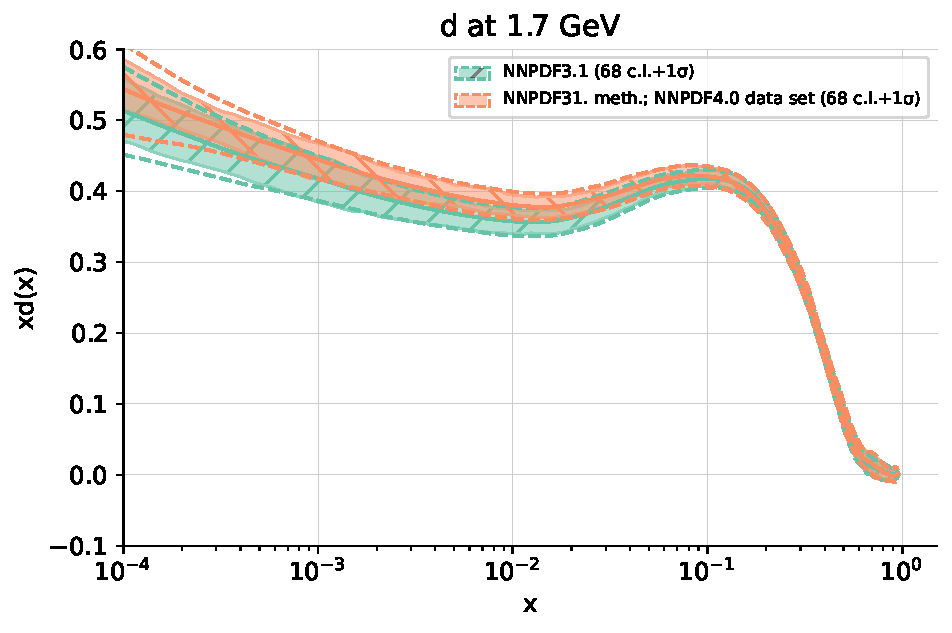
\includegraphics[width=\columnwidth]{plots/d_fit_2}\\    
    }
   \end{overlayarea}   
  \end{column} 
 \end{columns}
 \begin{columns}[c]
  \begin{column}{0.5\textwidth}
   \begin{overlayarea}{\columnwidth}{4cm}
    \only<1>
    {
     \centering
     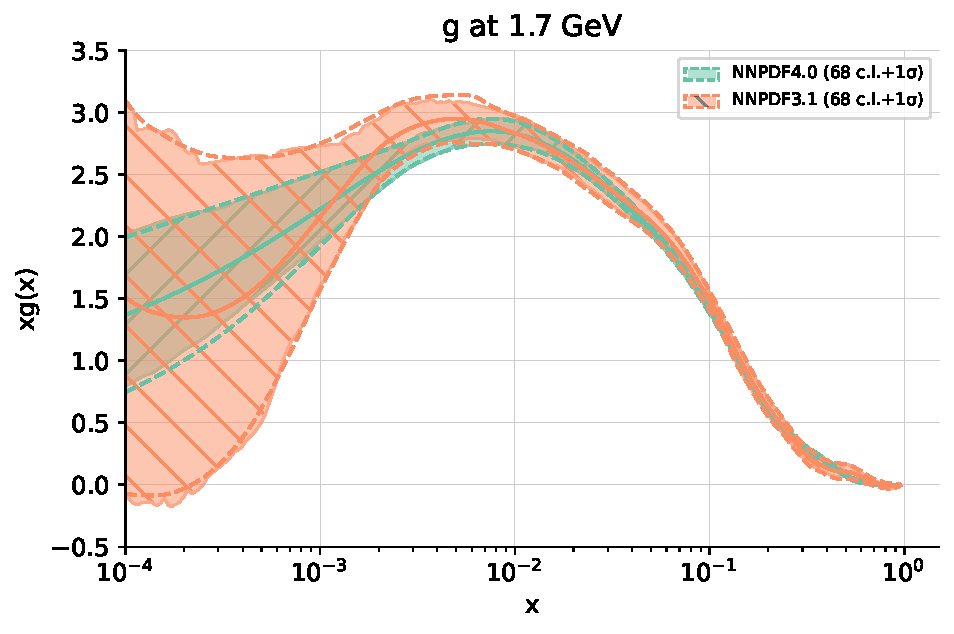
\includegraphics[width=\columnwidth]{plots/gluon_fit_1}\\
    }
    \only<2>
    {
     \centering
     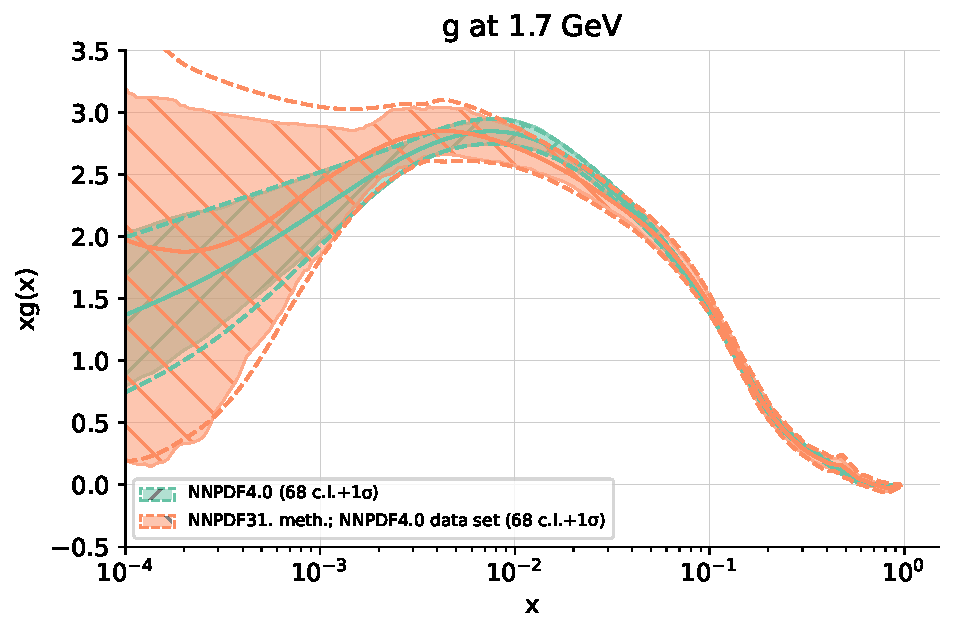
\includegraphics[width=\columnwidth]{plots/gluon_fit_2}\\    
    }
   \end{overlayarea}   
  \end{column}
  \begin{column}{0.5\textwidth}
   \begin{overlayarea}{\columnwidth}{4cm}
    \only<1>
    {
     \centering
     \tiny
     \renewcommand*{\arraystretch}{1.35}
     \begin{tabular}{lcc}
      \toprule
       \backslashbox{data set ($N_{\rm dat}$)}{methodology} & NNPDF3.1         & NNPDF4.0        \\
       \midrule
       NNPDF3.1 (4093)                                     & \alert{\bf 1.19} &            1.12  \\
       NNPDF4.0 (4491)                                     &      1.25        & \alert{\bf 1.17} \\
      \bottomrule
     \end{tabular}\\
     \vspace{0.3cm}
     \scriptsize
     \underline{Consistency} between PDF sets\\
     \vspace{0.2cm}
     NNPDF4.0 \underline{more precise}\\
     (combination of data set and methodology)\\
     \vspace{0.2cm}
     NNPDF4.0 \underline{more accurate}\\
     (superiority of the NNPDF4.0 methodology)\\
    }
    \only<2>
    {
      \centering
     \tiny
     \renewcommand*{\arraystretch}{1.35}
     \begin{tabular}{lcc}
      \toprule
       \backslashbox{data set ($N_{\rm dat}$)}{methodology} & NNPDF3.1         & NNPDF4.0        \\
       \midrule
       NNPDF3.1 (4093)                                      &            1.19  &            1.12  \\
       NNPDF4.0 (4491)                                      & \alert{\bf 1.25} & \alert{\bf 1.17} \\
      \bottomrule
     \end{tabular}\\
     \vspace{0.3cm}
     \scriptsize
     \underline{Consistency} between PDF sets\\
     \vspace{0.2cm}
     NNPDF4.0 \underline{more precise}\\
     (combination of data set and methodology)\\
     \vspace{0.2cm}
     NNPDF4.0 \underline{more accurate}\\
     (superiority of the NNPDF4.0 methodology)\\  
    }
   \end{overlayarea}   
  \end{column}   
 \end{columns}
\end{frame}

%Slide08
\begin{frame}
 \frametitle{The gluon PDF: impact of data}
 \footnotesize
 \centering
 \vspace{0.1cm}
 \begin{columns}[c]
  \begin{column}{0.5\textwidth}
   \centering
   jet and $t\bar{t}$ data\\
   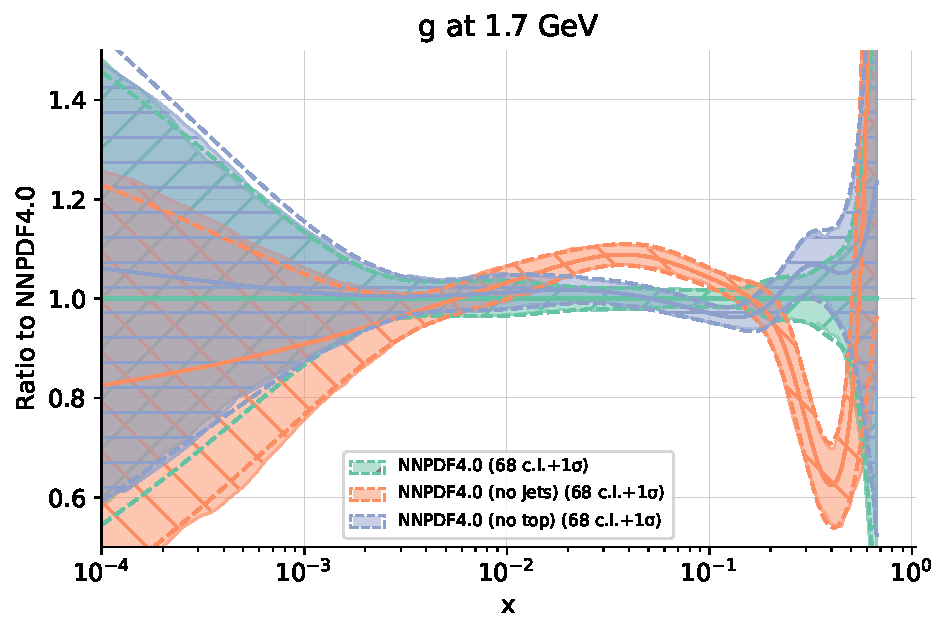
\includegraphics[width=\columnwidth]{plots/gluon_1}\\
  \end{column}
  \begin{column}{0.5\textwidth}
   \centering
   $Zp_T$ and direct photon data\\
   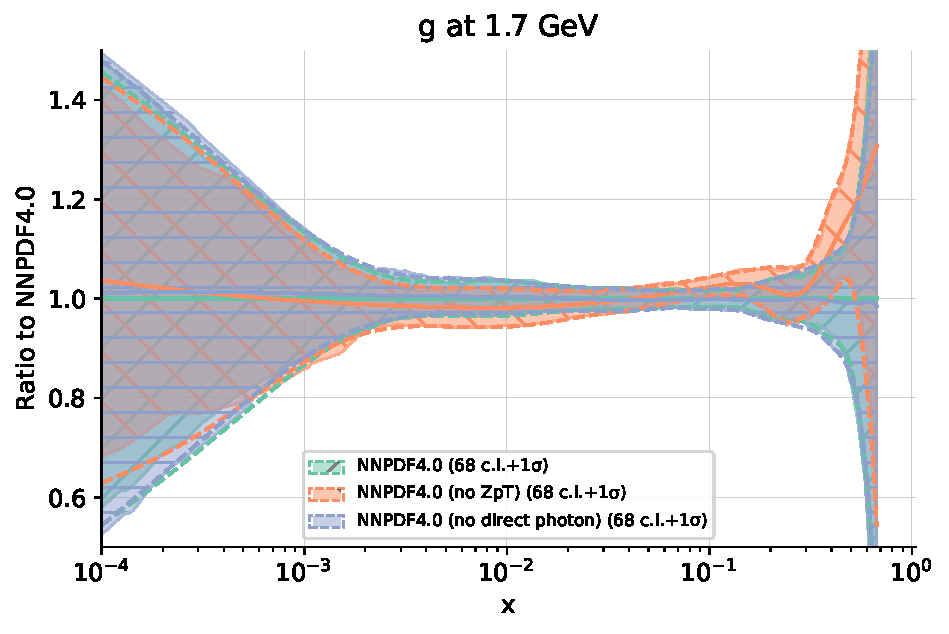
\includegraphics[width=\columnwidth]{plots/gluon_2}\\ 
  \end{column}
 \end{columns}
 %\vspace{0.2cm}
 Hierarchical impact of different data sets in the fit\\
 {\scriptsize jet measurements have the largest pull: suppression for $0.01\lesssim x\lesssim 0.1$, enhancement otherwise}\\ 
 {\scriptsize $t\bar{t}$ and $Zp_T$ measurements have a comparatively small pull, which is consistent with the global fit}\\
 {\scriptsize direct photon measurements have an almost immaterial pull}\\
 \vspace{0.1cm}
 \tiny
 \renewcommand*{\arraystretch}{1.15}
 \begin{tabularx}{\textwidth}{Xcccccccc}
  \toprule
  \backslashbox{fit}{data set} & ATLAS jets & CMS jets & ATLAS top & CMS top & ATLAS $Z p_T$ & CMS $Z p_T$ & ATLAS dir. phot. & total\\
  \midrule
  NNPDF4.0        &  1.06  &  1.55  &  2.29  &  0.77  &  0.86  &  1.41  &  0.71  & 1.17 \\
  (no jets)       & [1.71] & [3.70] &  1.54  &  1.00  &  0.86  &  1.35  &  0.72  & 1.14 \\
  (no top)        &  1.08  &  1.57  & [3.51] & [0.91] &  0.86  &  1.43  &  0.74  & 1.18 \\
  (no $Zp_T$)     &  1.08  &  1.57  &  2.30  &  0.76  & [0.99] & [1.41] &  0.69  & 1.14 \\
  (no dir. phot.) &  1.06  &  1.55  &  2.30  &  0.77  &  0.86  &  1.42  & [0.71] & 1.18 \\
  \bottomrule
 \end{tabularx}
\end{frame}

%Slide09
\begin{frame}
 \frametitle{The gluon PDF: single-inclusive jet vs di-jet data}
 \footnotesize
 \centering
 Inclusion of di-jet measurements is preferred over single-inclusive jet measurements\\
 given their greater theoretical accuracy and the avoidance of decorrelation models\\
 {\scriptsize based on an extensive study in the framework of the NNPDF3.1 methodology~{\tiny{[{\color{salmon}{EPJ C80 (2020) 8}}]}}}\\
 \vspace{0.2cm}
 \begin{columns}[c]
  \begin{column}{0.5\textwidth}
   \centering
   NNPDF3.1\\
   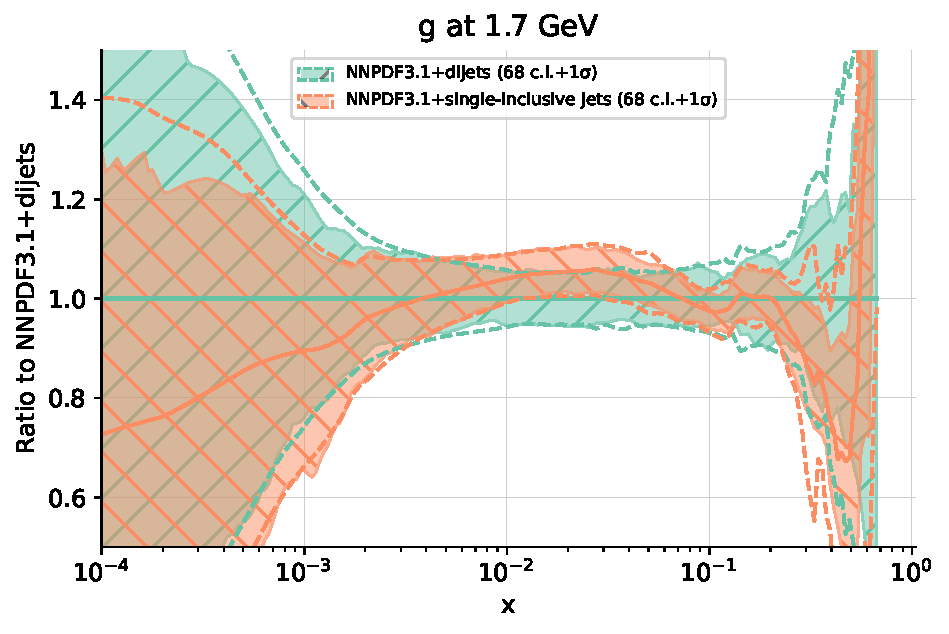
\includegraphics[width=\columnwidth]{plots/gluon_3}\\
  \end{column}
  \begin{column}{0.5\textwidth}
   \centering
   NNPDF4.0\\
   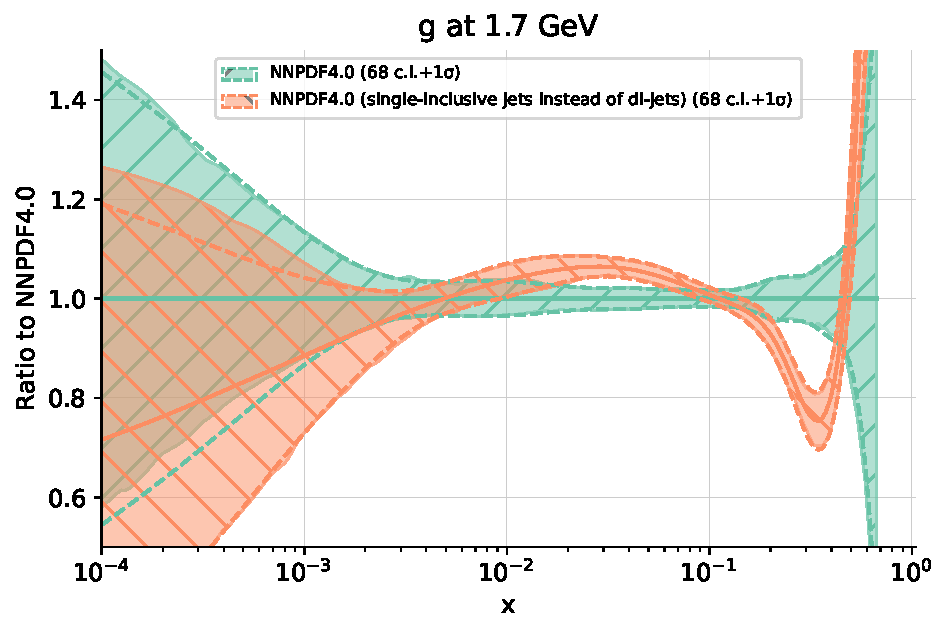
\includegraphics[width=\columnwidth]{plots/gluon_4}\\ 
  \end{column}
 \end{columns}
 Similar relative effect of single-inclusive vs di-jet data in NNPDF3.1 and NNPDF4.0\\
 \vspace{0.1cm}
 Effect enhanced within the reduced NNPDF4.0 uncertainties\\
 \vspace{0.1cm}
 \tiny
 \renewcommand*{\arraystretch}{1.15}
 \begin{tabularx}{\textwidth}{Xccccccccc}
  \toprule
  \backslashbox{fit}{data set}     & ATLAS 2j & CMS 2j & ATLAS 1j (7~TeV) & ATLAS 1j (8~TeV) & CMS 1j & $Z p_T$ & top & total\\
  \midrule
  NNPDF4.0                         &  1.93  &  1.56  & [1.28] [3.42]$^*$ & 0.61 [2.82]$^*$ & [1.31]  &  0.99  &  1.17  &  1.17 \\
  (single-jets instead of di-jets) & [2.41] & [2.68] & {\color{white}{[}}1.23{\color{white}{]}} [3.36]$^*$ & 0.85 [3.10]$^*$ &  1.07   &  0.99  &  1.19  &  1.14 \\
  \bottomrule
  $^*$No decorrelation model & \\
 \end{tabularx}
\end{frame}

%Slide10
\begin{frame}
 \frametitle{Quark flavour decomposition: impact of data}
 \footnotesize
 \begin{overlayarea}{\textwidth}{5.5cm}
  \only<1>
  {
   \centering
   Quarks\\
   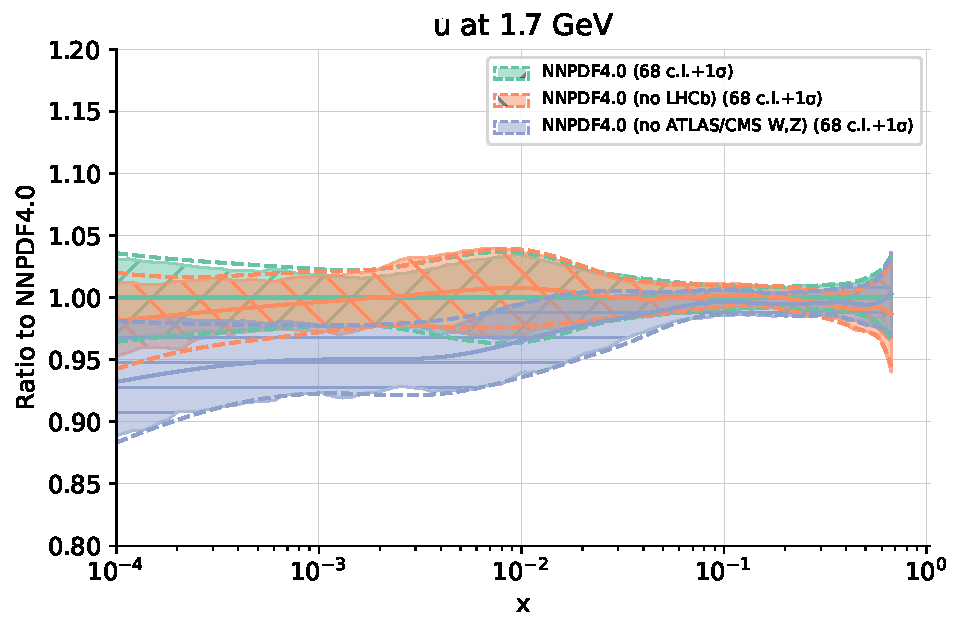
\includegraphics[width=0.48\textwidth]{plots/flavour_u}
   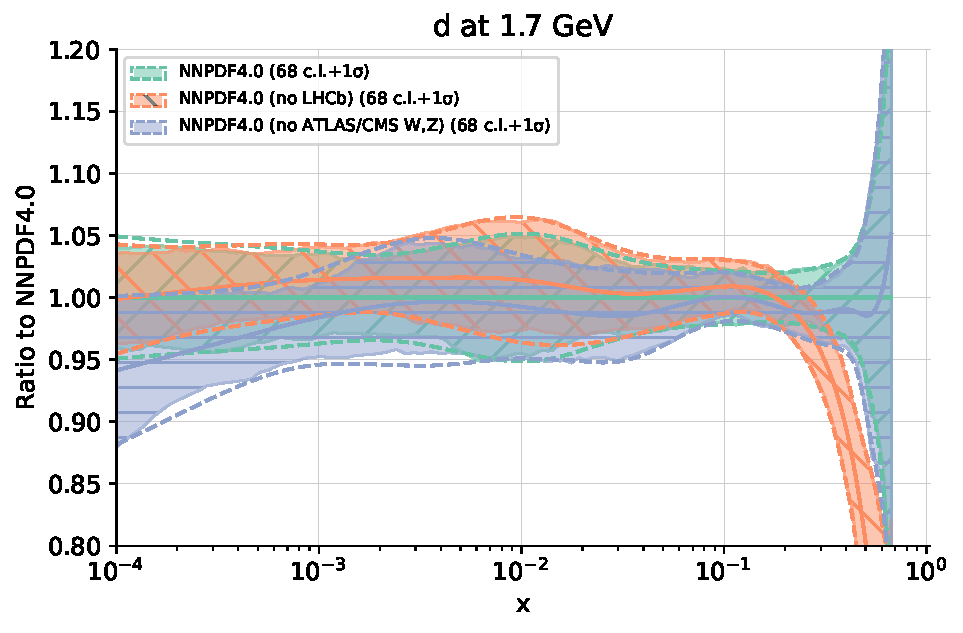
\includegraphics[width=0.48\textwidth]{plots/flavour_d}\\
   \vspace{0.1cm}
   The bulk of the constraint on $u$ and $d$ comes from inclusive fixed-target and collider DIS\\
   \vspace{0.1cm}
   LHCb data sets affect the $d$ PDF at large $x$ (as in NNPDF3.1)\\
   \vspace{0.1cm}
   Effect of single top (not shown) is immaterial, see~{\tiny{[{\textcolor{salmon}{JHEP\,05\,(2020)\,067}}]}}\\
  }
  \only<2>
  {
   \centering
   Antiquarks\\
   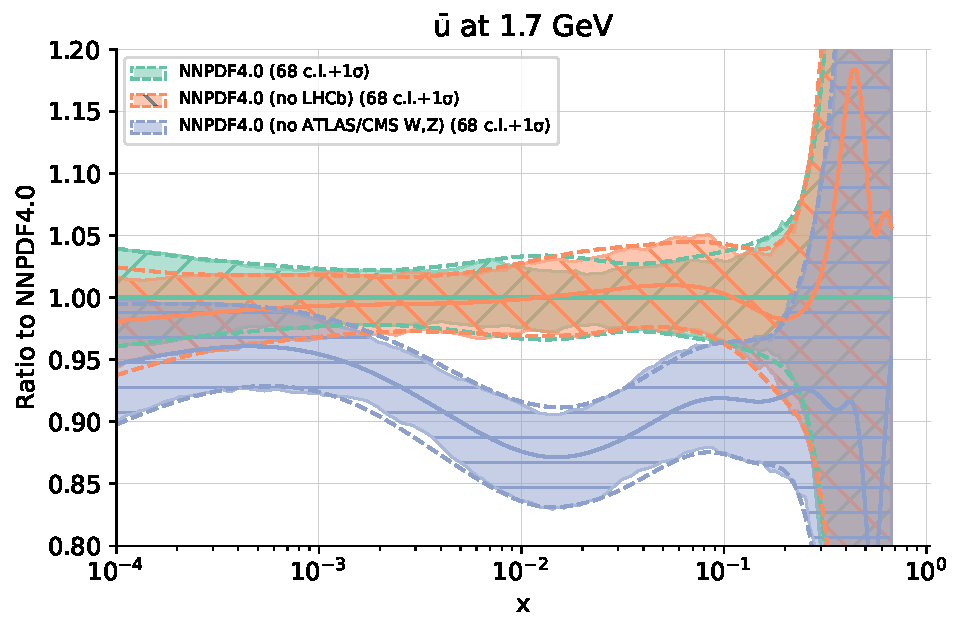
\includegraphics[width=0.48\textwidth]{plots/flavour_baru}
   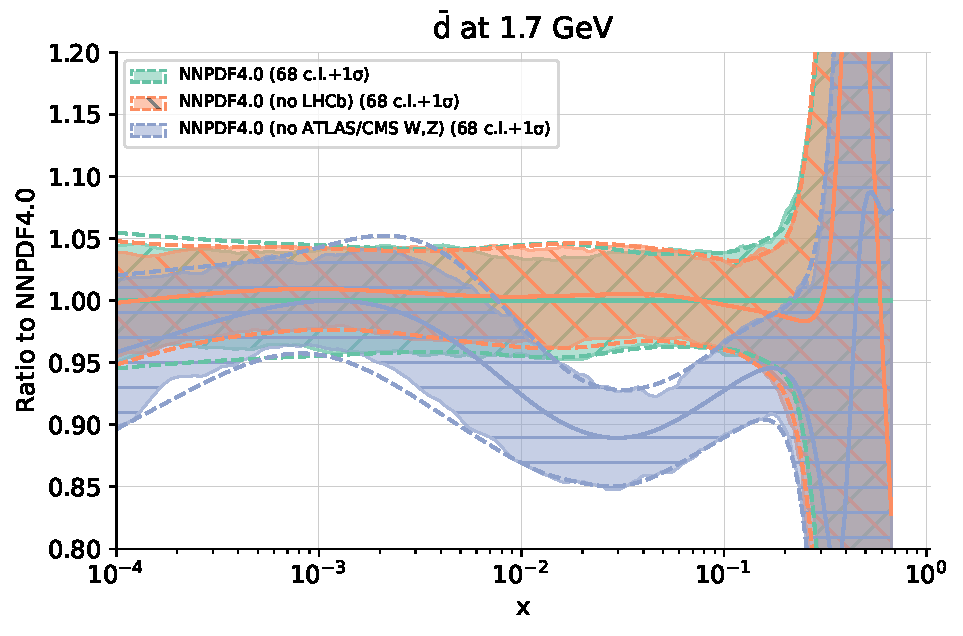
\includegraphics[width=0.48\textwidth]{plots/flavour_bard}\\
   ATLAS and CMS DY data sets have a pull of about $2\sigma$ for $x\sim 0.02$ on both $\bar{u}$ and $\bar{d}$\\
   \vspace{0.1cm}
   The pull is not encompassed by a corresponding increase of PDF uncertainties\\
   \vspace{0.1cm}
   Genuine effect of data, detected thanks to the new methodology and data set\\
  }
 \end{overlayarea}
 \vspace{0.4cm}
 \tiny
 \renewcommand*{\arraystretch}{1.15}
 \begin{tabularx}{\textwidth}{Xccccccccc}
  \toprule
  \backslashbox{fit}{data set}     & FT DIS & HERA & FT DY & Tevatron & ATLAS $W,Z$ & CMS $W,Z$ & LHCb & single top & total\\
  \midrule
  NNPDF4.0                         & 1.10 & 1.21 &  1.00  &  1.14  &  1.28  &  1.33  &  1.54  &  0.37  & 1.17 \\
  (no LHCb)                        & 1.08 & 1.21 &  0.97  &  1.27  &  1.34  &  1.35  & [2.60] &  0.34  & 1.16 \\      
  (no ATLAS/CMS $W,Z$)             & 1.05 & 1.20 &  0.85  &  1.02  & [2.14] & [1.36] &  1.39  &  0.37  & 1.11 \\
  \midrule
  DIS-only                         & 1.03 & 1.21 & [1.40] & [1.22] & [4.15] & [3.83] & [2.96] & [0.33] & 1.10 \\
  \bottomrule
 \end{tabularx} 
\end{frame}

%Slide11
\begin{frame}
 \frametitle{Quark flavour separation: nuclear uncertainties}
 \footnotesize
 \centering
 \begin{columns}[c]
  \begin{column}{0.5\textwidth}
   \centering
   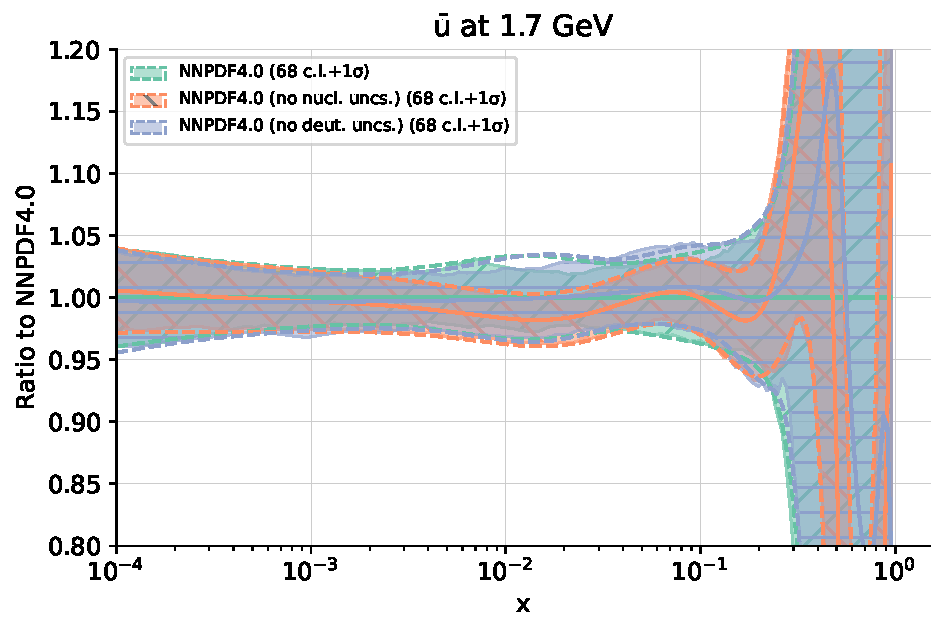
\includegraphics[width=\columnwidth]{plots/nuclear_baru}\\
  \end{column}
  \begin{column}{0.5\textwidth}
   \centering
   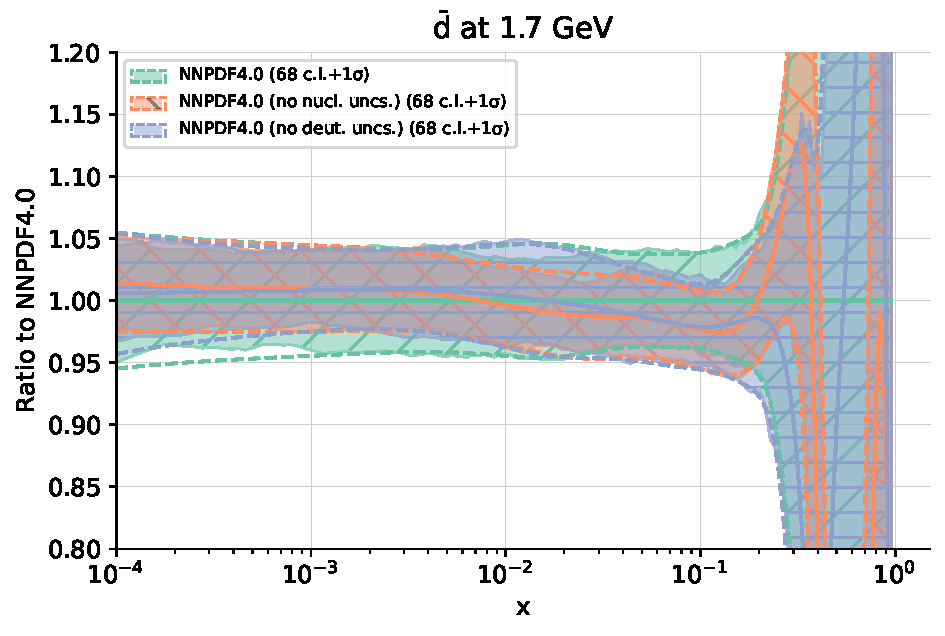
\includegraphics[width=\columnwidth]{plots/nuclear_bard}\\
  \end{column}
 \end{columns}
  \begin{columns}[c]
  \begin{column}{0.5\textwidth}
   \centering
   Effect of nuclear uncertainties relevant\\ at large $x$\\
   to reconcile FT DIS with LHC DY data\\
   \vspace{0.1cm}
   {\scriptsize $\chi^2_{\rm tot}=1.17\to \chi^2_{\rm tot}=1.26$ (no nucl. uncs.)}\\
   {\scriptsize $\chi^2_{\rm LHCb}=1.54\to \chi^2_{\rm tot}=1.76$ (no nucl. uncs.)}\\
   \vspace{0.2cm}
   The bulk of the effect is due to nuclear uncertainties for heavy nuclei\\
   {\scriptsize deuteron uncertainties have a comparatively smaller effect at inermediate values of $x$}\\
  \end{column}
  \begin{column}{0.5\textwidth}
   \centering
   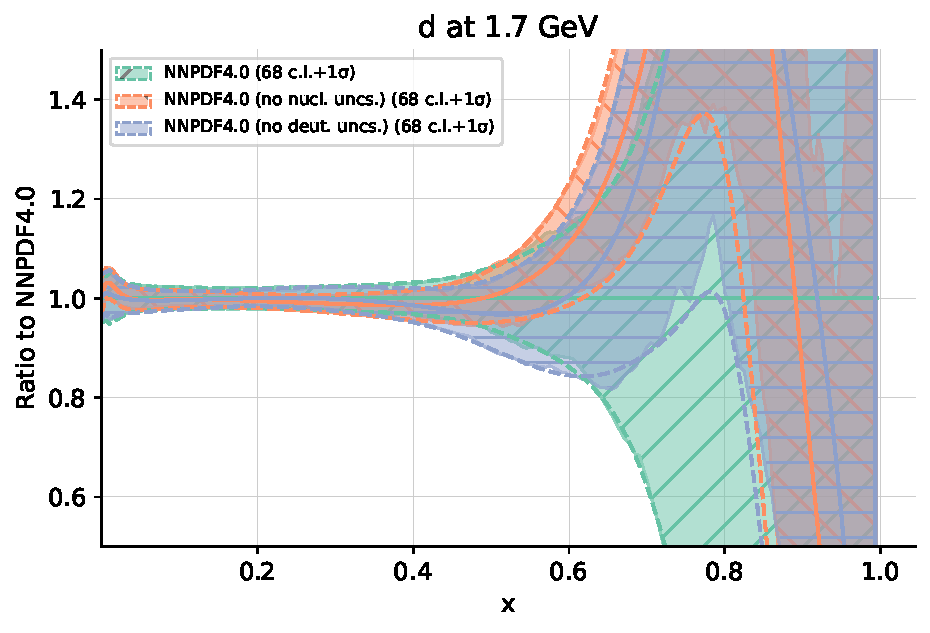
\includegraphics[width=\columnwidth]{plots/nuclear_d}\\   
  \end{column}
 \end{columns}
\end{frame}

%Slide12
\begin{frame}
 \frametitle{The strange PDF: impact of data}
 \footnotesize
 \centering
 \begin{columns}[c]
  \begin{column}{0.5\textwidth}
   \centering
   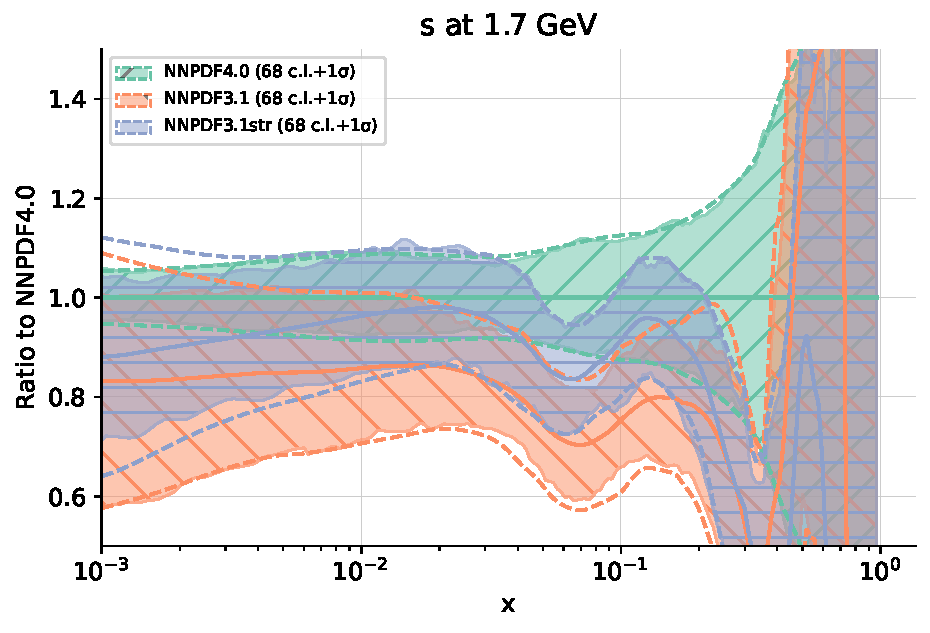
\includegraphics[width=\columnwidth]{plots/strange_1}\\
  \end{column}
  \begin{column}{0.5\textwidth}
   \centering
   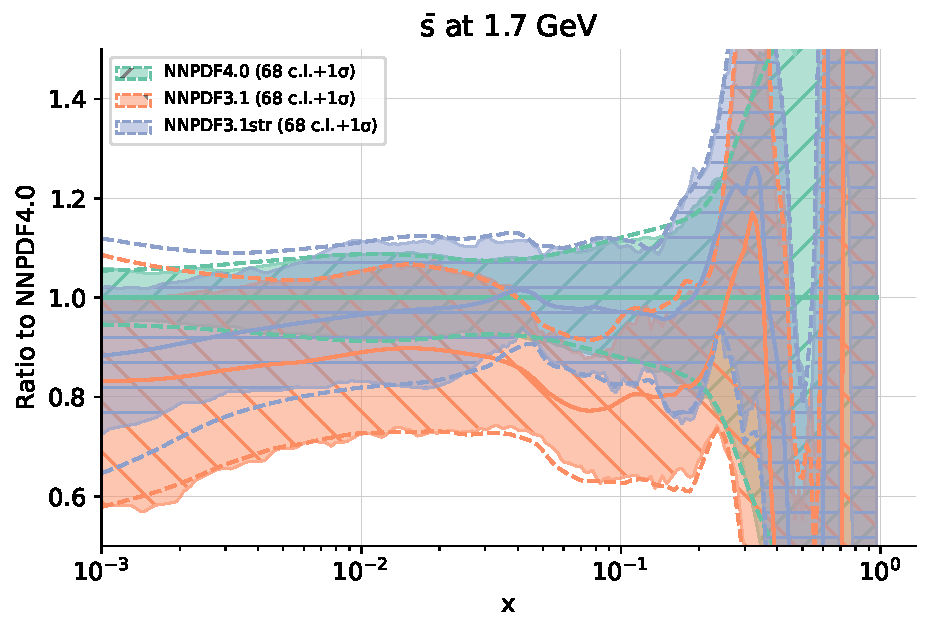
\includegraphics[width=\columnwidth]{plots/strange_2}\\
  \end{column}
 \end{columns}
 \begin{columns}[c]
  \begin{column}{0.5\textwidth}
   \centering
   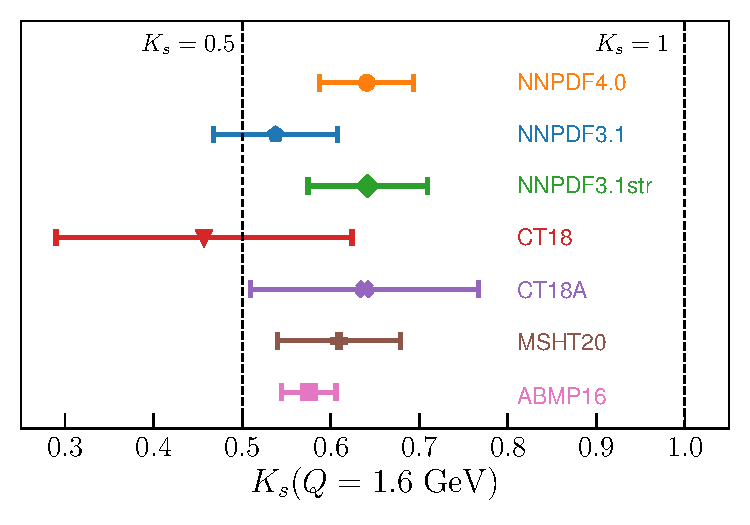
\includegraphics[width=\columnwidth]{plots/ks-Q_1p6GeV}\\
  \end{column}
  \begin{column}{0.5\textwidth}
   \centering
   \footnotesize
   Enhanced $s$ and $\bar{s}$ PDFs w.r.t. NNPDF3.1\\
   {\scriptsize effect of ATLAS $W,Z$ and $W$+jet data}\\
   \vspace{0.2cm}
   Good consistency with NNPDF3.1str\\
   {\scriptsize no nuclear uncertainties in NNPDF3.1str}\\
   {\scriptsize no NOMAD data in NNPDF4.0}\\
   \vspace{0.2cm}
   Good consistency of $K_s$ across PDF sets\\ 
   \vspace{0.1cm}
   $K_s(Q^2)=\frac{\int_0^1\,dx[s(x,Q^2)+\bar{s}(x,Q^2)]}{\int_0^1\,dx[\bar{u}(x,Q^2)+\bar{d}(x,Q^2)]}$\\
   \begin{flushright}
    {\tiny{See also [{\color{salmon}{EPJ\,C80\,(2020)\,1168}}]}}
   \end{flushright}
  \end{column}
 \end{columns} 
\end{frame}

%Slide13
\begin{frame}
 \frametitle{Impact of theory: perturbative vs fitted charm}
 \footnotesize
 \centering
 \begin{columns}[c]
  \begin{column}{0.5\textwidth}
   \centering
   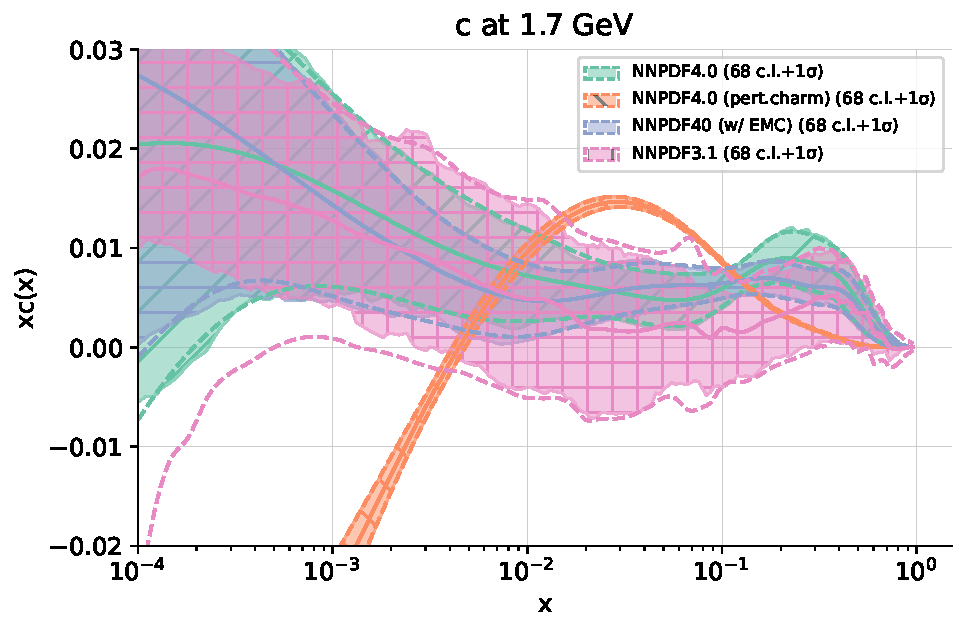
\includegraphics[width=\columnwidth]{plots/charm_1}\\
  \end{column}
  \begin{column}{0.5\textwidth}
   \centering
   Striking evidence of intrinsic charm\\
   {\scriptsize even w/o EMC $F_2^c$ data}\\
   \vspace{0.2cm}
   Perturbative charm alters the flavour decomposition and deteriorates the fit\\
   \vspace{0.1cm}
   {\scriptsize $\chi^2_{\rm fitted\,charm}=1.17\to \chi^2_{\rm pert.\,charm}=1.19$}\\
   \vspace{0.2cm}
   {\scriptsize mainly due to a worsening\\ of the LHC $W,Z$ and top pair data sets}\\
  \end{column}
 \end{columns}
 \begin{columns}[c]
  \begin{column}{0.5\textwidth}
   \centering
   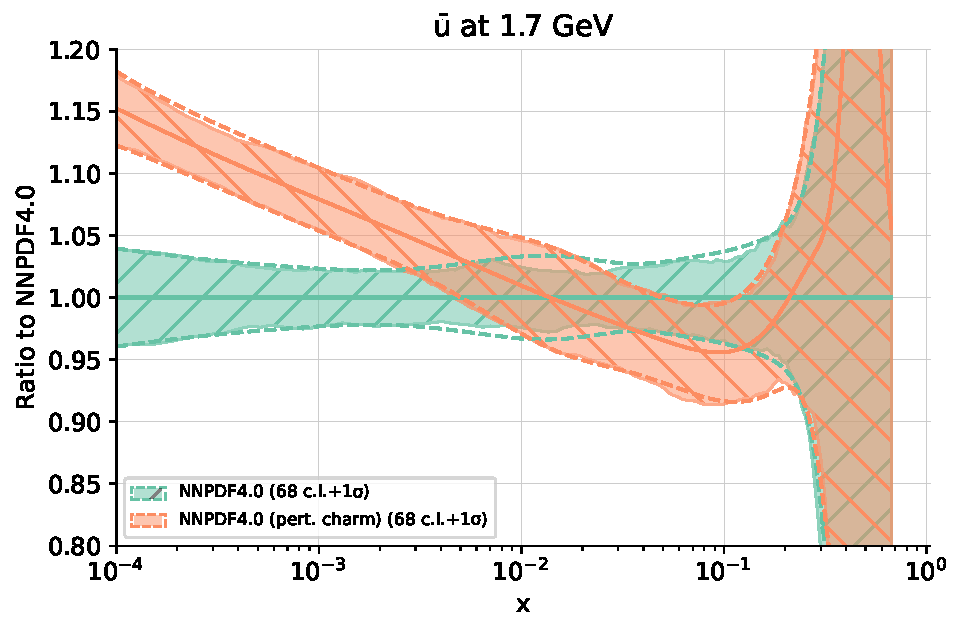
\includegraphics[width=\columnwidth]{plots/charm_2}\\
  \end{column}
  \begin{column}{0.5\textwidth}
   \centering
   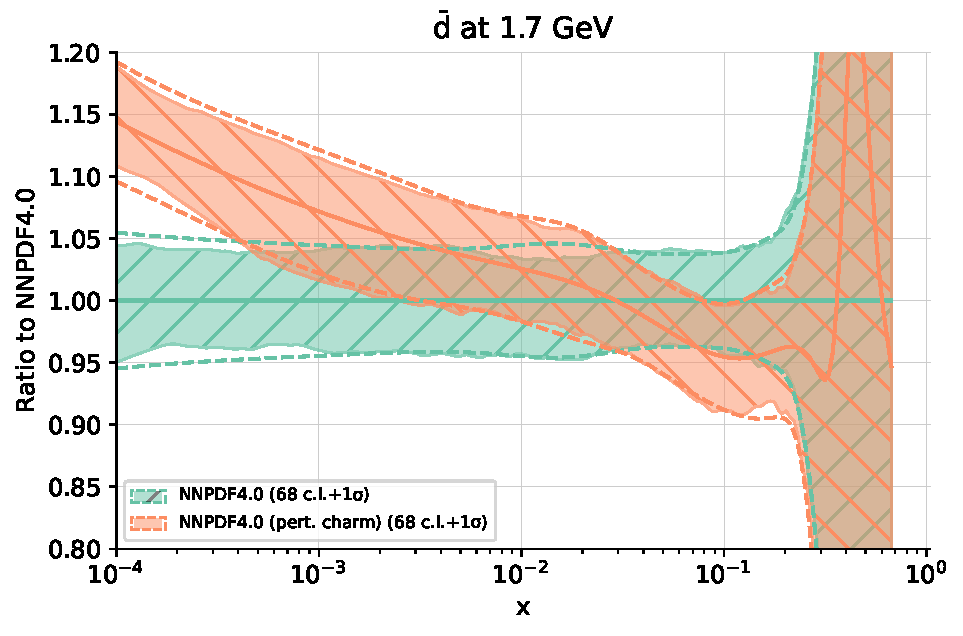
\includegraphics[width=\columnwidth]{plots/charm_3}\\
  \end{column}
 \end{columns}
\end{frame}

%Slide14
\begin{frame}
 \frametitle{NNPDF4.0: parton luminosities}
 \footnotesize
 \centering
 \begin{overlayarea}{\textwidth}{10cm}
  \only<1>
  {
   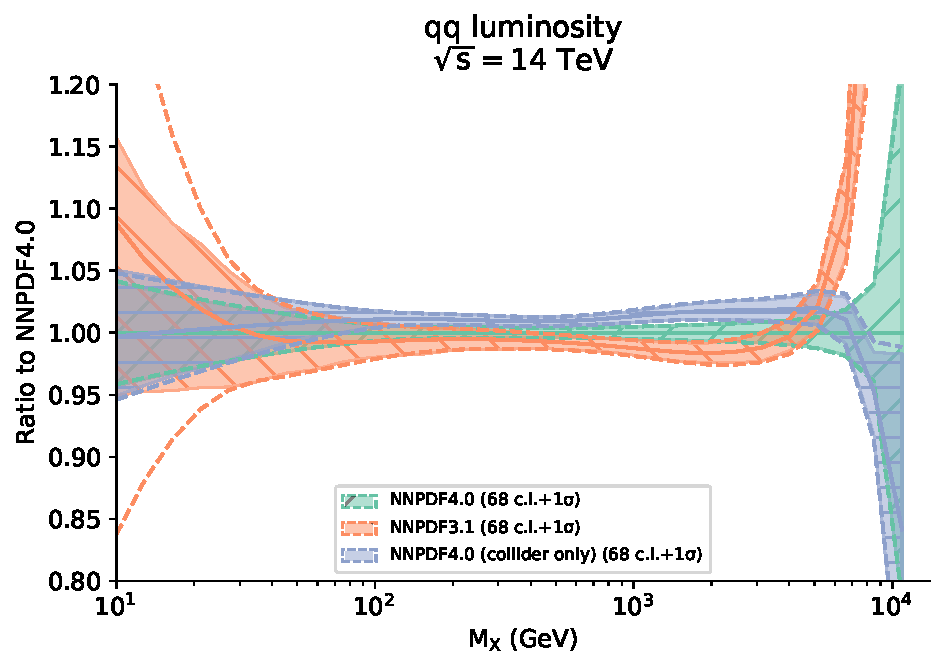
\includegraphics[width=0.48\textwidth]{plots/lumi_qq_1}
   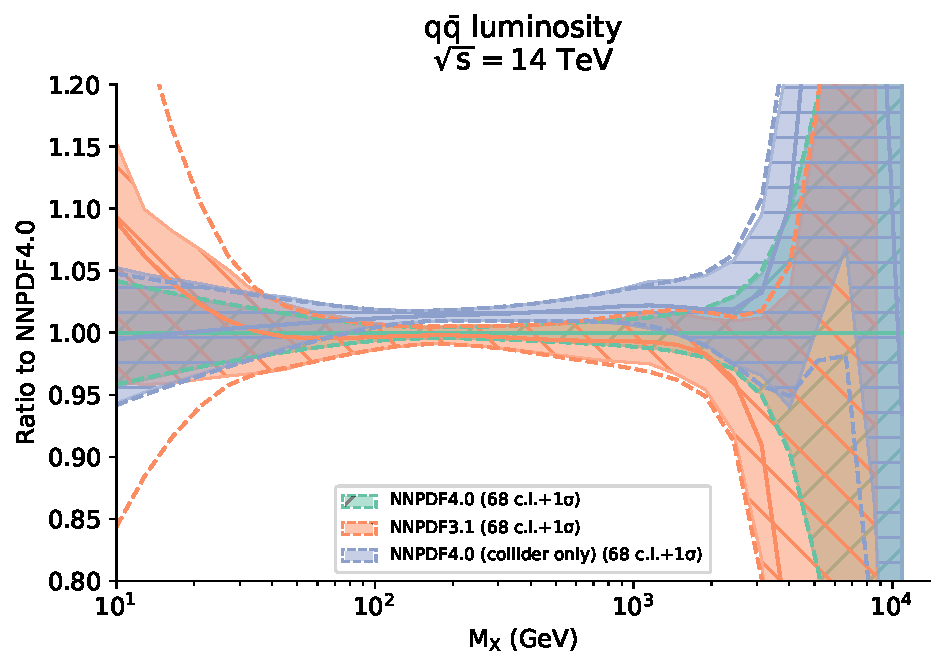
\includegraphics[width=0.48\textwidth]{plots/lumi_qqbar_1}\\
   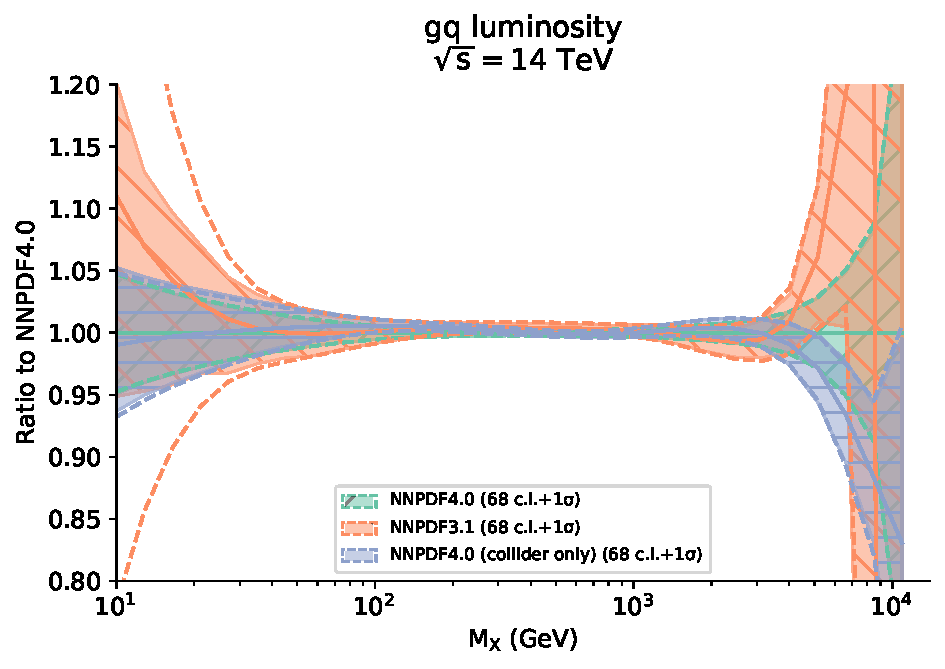
\includegraphics[width=0.48\textwidth]{plots/lumi_gq_1}
   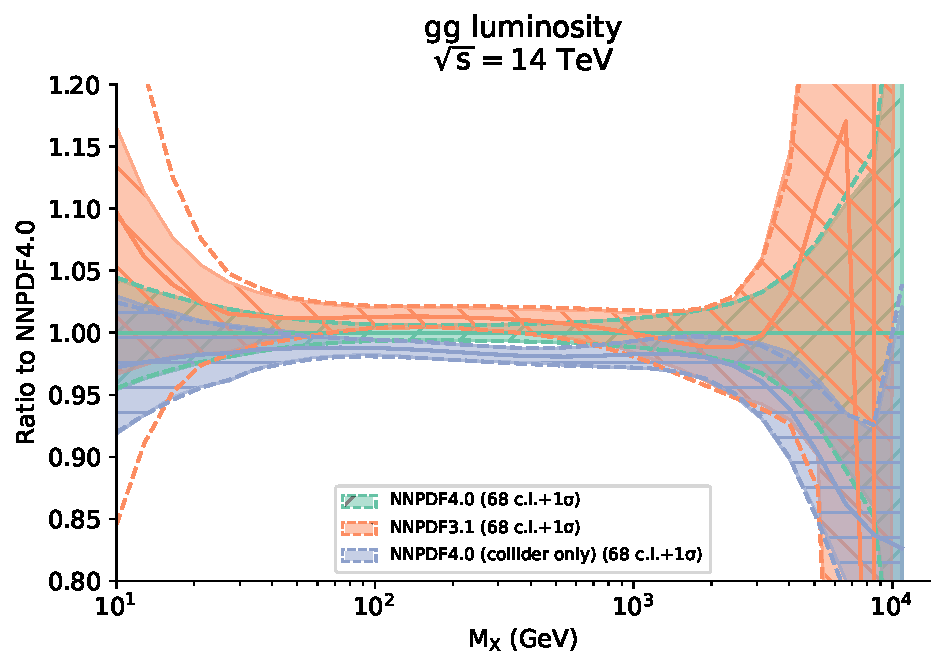
\includegraphics[width=0.48\textwidth]{plots/lumi_gg_1}\\
  }
  \only<2>
  {
   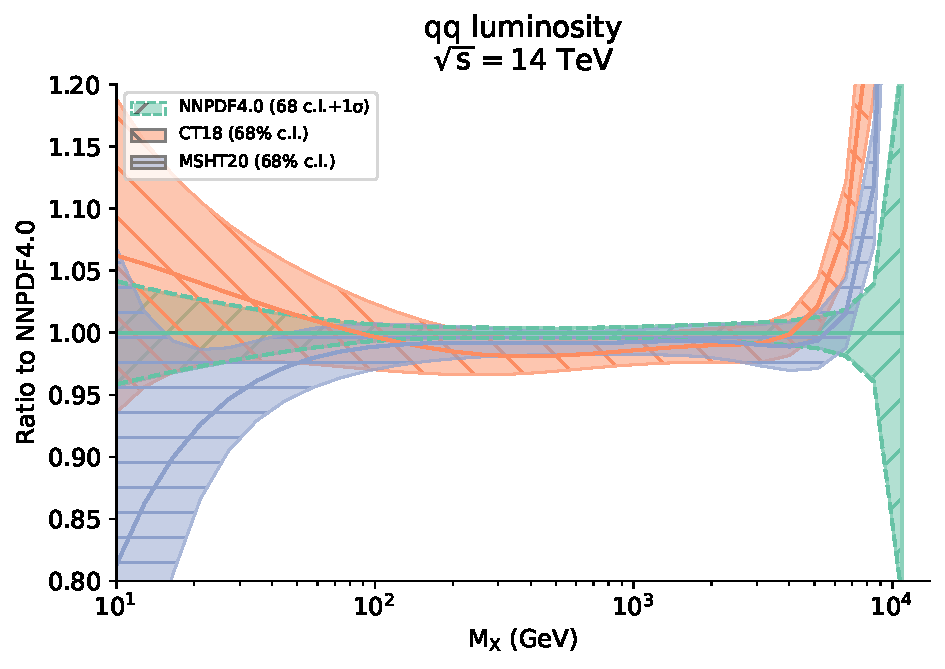
\includegraphics[width=0.48\textwidth]{plots/lumi_qq_2}
   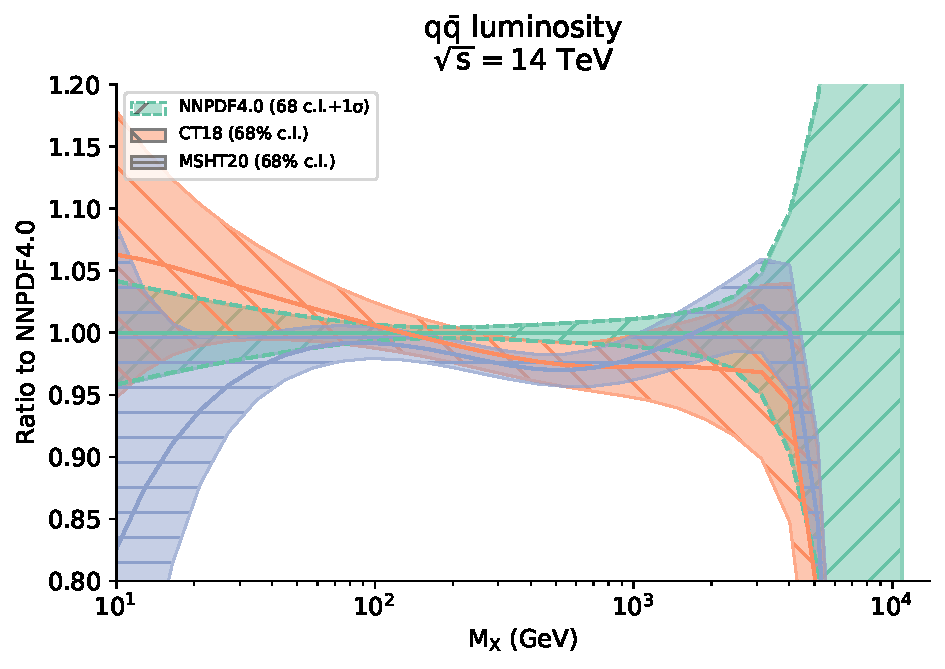
\includegraphics[width=0.48\textwidth]{plots/lumi_qqbar_2}\\
   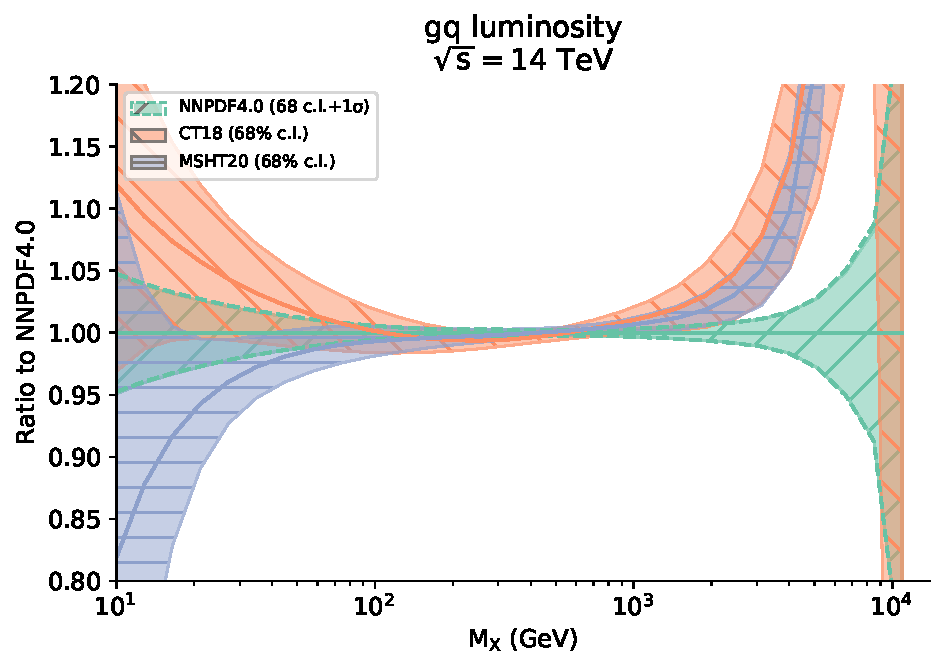
\includegraphics[width=0.48\textwidth]{plots/lumi_gq_2}
   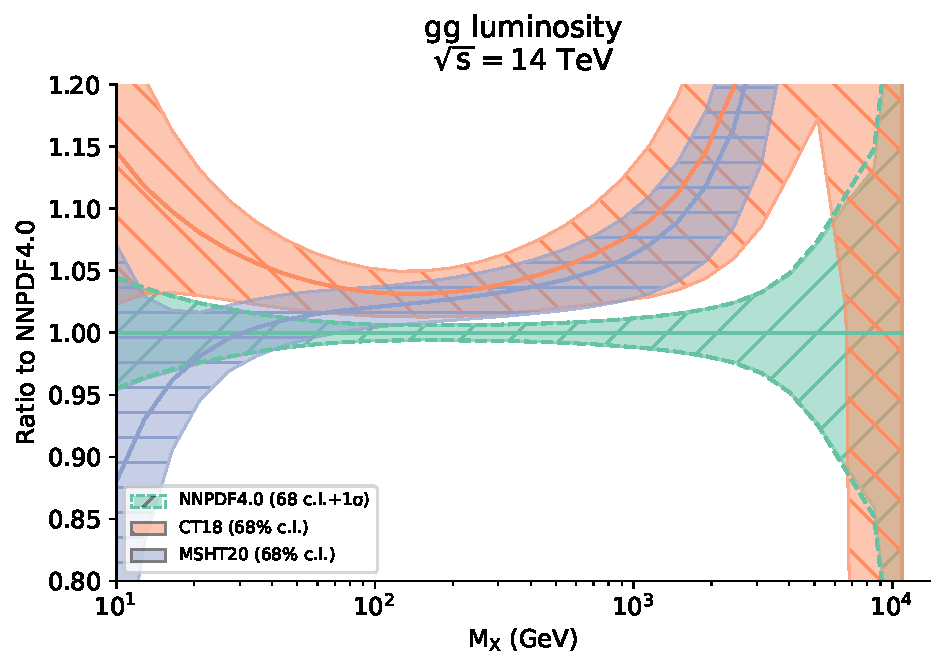
\includegraphics[width=0.48\textwidth]{plots/lumi_gg_2}\\  
  }
 \end{overlayarea}
\end{frame}

%Slide15
\begin{frame}
 \frametitle{NNPDF4.0: implications for LHC phenomenology}
 \footnotesize
 \centering
 \vspace{0.2cm}
 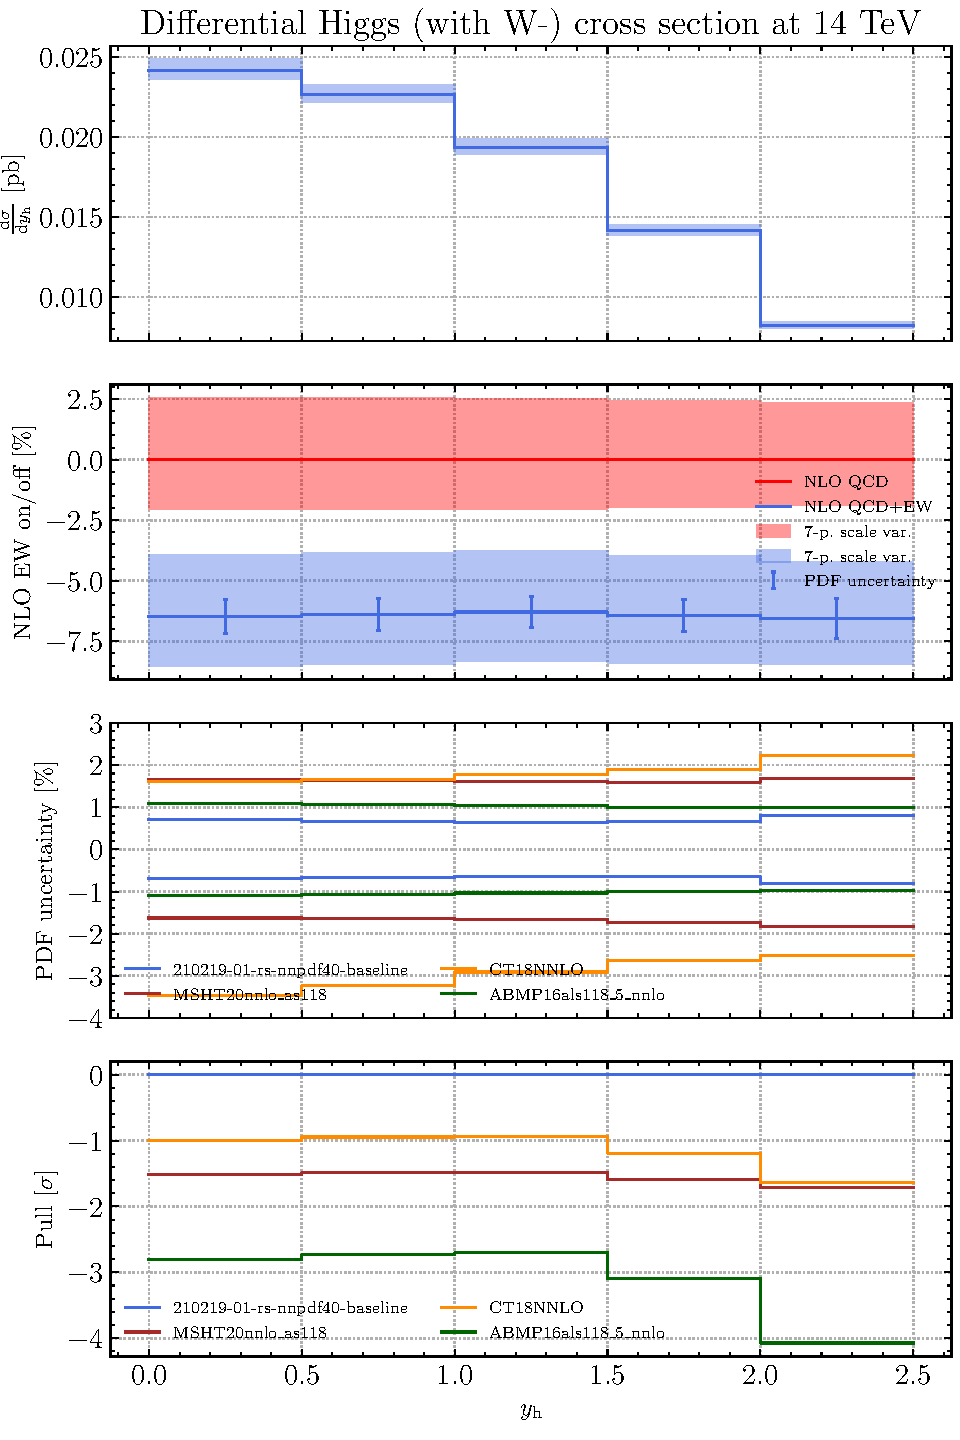
\includegraphics[width=0.43\textwidth]{plots/NNPDF40_HIGGS_WM-global}
 \ \ \ \ \ \ \ \ \ 
 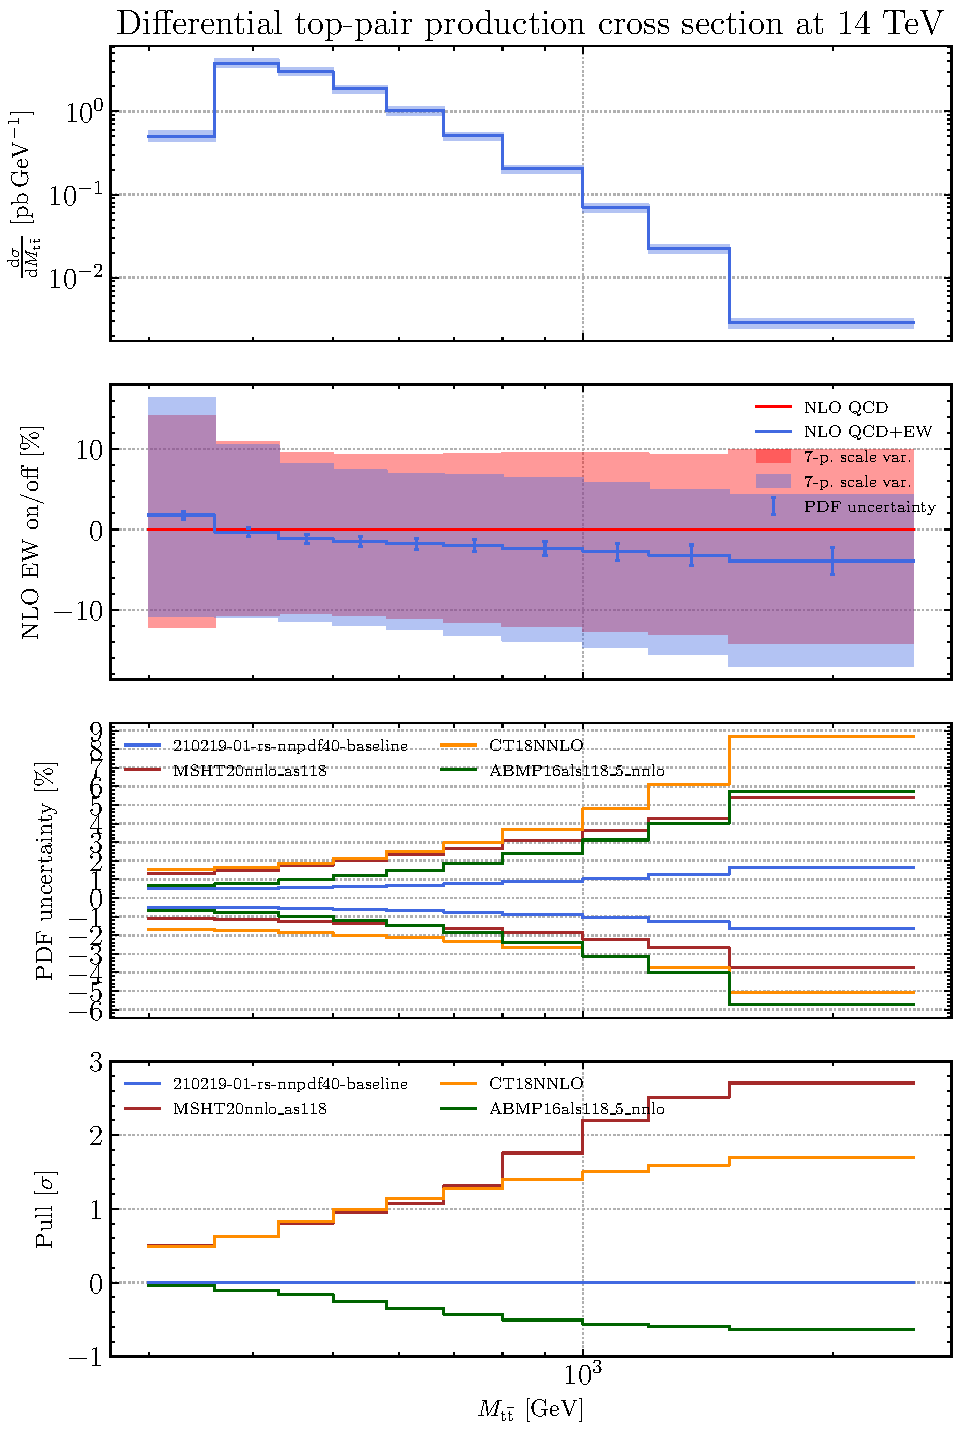
\includegraphics[width=0.43\textwidth]{plots/NNPDF40_TTBAR-global}\\
 \begin{flushright}
  \tiny{[{\color{salmon}{Plots by courtesy of C.~Schwan}}]}
 \end{flushright}
\end{frame}

%Slide16
\begin{frame}
 \frametitle{Conclusions}
 \footnotesize
 \centering
 NNPDF4.0 is the next generation parton set of the NNPDF family\\
 \vspace{0.3cm}
 It achieves 1\% accuracy in an unprecedentedly broad kinematic range\\
 by consistently improving the previous NNPDF3.1 parton set\\
 \vspace{0.3cm}
 This result builds upon an extensive LHC data set\\ 
 combined with deep-learning optimisation models\\
 \vspace{0.3cm}
 Its faithfulness in representing PDF uncertainties is completely validated by closure tests\\
 \vspace{0.3cm}
 1\% PDF uncertainties challenge the accuracy of theoretical predictions\\
 and demand an increasing effort towards the systematic inclusion of\\ 
 theoretical uncertainties (nuclear, high-order, physical parameters, \dots)\\
 and higher-order QCD and EW corrections\\
 \vspace{0.3cm}
 The NNPDF code used to produce the NNPDF4.0 parton set\\ 
 will be made publicly available with its documentation\\
 \vspace{1cm}
 \begin{overlayarea}{\textwidth}{0.5cm}
  \only<1>
  {
  }
  \only<2>
  {
  \centering
  \Large\bf Thank you
  }
 \end{overlayarea}
\end{frame}

\end{document}



